\chapter{Zero-free Regions \& Zero Counting of \texorpdfstring{$L$}{L}-functions}
  In this chapter, we expand our discussion about the zeros of $L$-functions. We prove the classical zero-free regions for the Riemann zeta function and Dirichlet $L$-functions. In the latter case, we introduce the infamous Siegel zeros. After the zero-free regions, we discuss zero counting up the critical strip. The main result we prove is the Riemann–von Mangoldt formula and its analog for Dirichlet $L$-functions.
  \section{The Explicit Formula for Logarithmic Derivatives}
    Information about the distribution of primes is ultimatiely contained in the information about the zeros of the $L$-functions $\z(s)$ and $L(s,\chi)$. In order to extract this information we will require more flexiable tools than the $L$-functions alone. These tools are explicit formulas for logarithmic derivatives of $L$-functions. Essentially, explicit formulas are partial fraction decomposition analogs to analytic functions. 
    \subsection*{The Explicit Formula for the Logarithmic Derivative of \texorpdfstring{$\z(s)$}{\z(s)}}
      Define the \textbf{Riemann xi function}\index{Riemann xi function} $\xi(s)$ by
      \[
        \xi(s) = \frac{1}{2}s(s-1)\pi^{-\frac{s}{2}}\G\left(\frac{s}{2}\right)\z(s).
      \]
      Note that $\xi(s)$ is holomorphic on $\C$ since at $s = 1$ the pole of $\z(s)$ is canceled by the zero from the $s(s-1)$ term and the poles coming from the gamma function are canceled by the trivial zeros of $\z(s)$ or by $s$ in the case $s = 0$. By the functional equation for $\z(s)$,
      \[
        \xi(s) = \xi(1-s),
      \]
      which is the functional equation for the Riemann xi function. Moreover, $\xi(s)$ is of order $1$. To see this, by the functional equation for the Riemann xi function it suffices to prove $\xi(s)$ is of order $1$ for $\Re(s) \ge \frac{1}{2}$. Now $\z(s)$ is of order $1$, being a Selberg class $L$-function, and $\G\left(\frac{s}{2}\right)$ is of order $1$ for $\Re(s) > 0$. By the Hadamard factorization theorem (see \cref{append:Factorizations_and_Finite_Order}),
      \begin{equation}\label{equ:Hadamard_product_for_Riemann_xi}
        \xi(s) = e^{A+Bs}\prod_{\rho}\left(1-\frac{s}{\rho}\right)e^{\frac{s}{\rho}},
      \end{equation}
      where $A$ and $B$ are constants and $\rho$ runs over the nontrivial zeros of $\z(s)$, counted with multiplicity, ordered with respect to the size of the ordinate. That is, if $\rho = \b+i\g$, the product is ordered by $|\g|$. \cref{equ:Hadamard_product_for_Riemann_xi} is an infinite product expression for $\xi(s)$ and we will use it to obtain the explicit formula for logarithmic derivative of $\z(s)$. To do this we tak the logarithmic derivative of $\xi(s)$ in two ways. First, observe that we can write $\xi(s) = (s-1)\pi^{-\frac{s}{2}}\G\left(\frac{s}{2}+1\right)\z(s)$. The logarithm derivative of this expression gives
      \begin{equation}\label{equ:logarithmic_derivative_Riemann_xi_1}
        \frac{\xi'}{\xi}(s) = \frac{1}{s-1}+\frac{1}{2}\log(\pi)+\frac{1}{2}\frac{\G'}{\G}\left(\frac{s}{2}+1\right)+\frac{\z'}{\z}(s).
      \end{equation}
      On the other hand, we can take the logarithmic derivative \cref{equ:Hadamard_product_for_Riemann_xi} to obtain
      \begin{equation}\label{equ:logarithmic_derivative_Riemann_xi_2}
        \frac{\xi'}{\xi}(s) = B+\sum_{\rho}\left(\frac{1}{s-\rho}+\frac{1}{\rho}\right).
      \end{equation}
      Upon combining \cref{equ:logarithmic_derivative_Riemann_xi_1,equ:logarithmic_derivative_Riemann_xi_2} yields the \textbf{explicit formula}\index{explicit formula} for $\frac{\z'}{\z}(s)$:
      \[
        \frac{\z'}{\z}(s) = B-\frac{1}{s-1}-\frac{1}{2}\log(\pi)-\frac{1}{2}\frac{\G'}{\G}\left(\frac{s}{2}+1\right)+\sum_{\rho}\left(\frac{1}{s-\rho}+\frac{1}{\rho}\right).
      \]
      The explicit formula for $\frac{\z'}{\z}(s)$ is quite important for analytic investigations. Notice that the second term contains information about the pole of $\z(s)$ while the last term contains all the information about the nontrivial zeros. The digamma function term contains the information about the trivial zeros as can be seen from \cref{cor:logarithmic_derivative_of_gamma}.

      The constants $A$ and $B$ in \cref{equ:Hadamard_product_for_Riemann_xi} can be computed. To compute $A$, \cref{equ:Hadamard_product_for_Riemann_xi} implies $A = \log(\xi(0))$. Now $\z(s)$ has residue $1$ at $s = 1$ so that $\lim_{s \to 1}(s-1)\z(s) = 1$. This fact along with $\G\left(\frac{1}{2}\right) = \sqrt{\pi}$ together imply $\xi(1) = \frac{1}{2}$. By the functional equation for $\xi(s)$, we find that
      \[
        A = \log\left(\frac{1}{2}\right).
      \]
      The constant $B$ requires slightly more work. We first claim that $\sum_{\rho}\frac{1}{\rho}$ converges provided we group the terms $\rho$ and $\conj{\rho}$ together. This is in accordance with the order of $\rho$ in the Hadamard factorization for $\xi(s)$. Letting $\rho = \b+i\g$, we have
      \begin{equation}\label{equ:B_computation_1}
        \sum_{\rho}\frac{1}{\rho} = \asum_{\rho}\left(\frac{1}{\rho}+\frac{1}{\conj{\rho}}\right) = \sum_{|\g| \ge 0}\frac{2\b}{\b^{2}+\g^{2}},
      \end{equation}
      where the $\ast$ indicates that we are summing over $\rho$ and not $\conj{\rho}$. The last sum in \cref{equ:B_computation_1} is at most $2\sum_{\rho}\frac{1}{|\rho|^{2}}$ and this sum converges by the Hadamard factorizaton of $\xi(s)$ since the rank is $1$. Now \cref{equ:logarithmic_derivative_Riemann_xi_2} and the functional equation for $\xi(s)$ together give
      \begin{equation}\label{equ:B_computation_2}
        B+\sum_{\rho}\left(\frac{1}{s-\rho}+\frac{1}{\rho}\right) = -B-\sum_{\rho}\left(\frac{1}{1-s-\rho}+\frac{1}{\rho}\right).
      \end{equation}
      The terms corresponding to $s-\rho$ and $1-s-\rho$ cancel because if $\rho$ is a nontrivial zero so is $1-\rho$. Indeed, add $\sum_{p}\frac{1}{1-s-\rho}$ to both sides of \cref{equ:B_computation_2} and notice that $\frac{1}{1-s-\rho} = -\frac{1}{s-(1-\rho)}$. Using \cref{equ:B_computation_1} we can rewrite the result as
      \[
        B = -\sum_{\rho}\frac{1}{\rho} = -\sum_{|\g| \ge 0}\frac{2\b}{\b^{2}+\g^{2}}.
      \]
    \subsection*{The Explicit Formula for the Logarithmic Derivative of \texorpdfstring{$L(s,\chi)$}{L(s,\chi)}}
      Let $\chi$ be a primitive Dirichlet character with conductor $q > 1$. We will derive an analogous explicit formula for the logarithmic derivative of $L(s,\chi)$. To do this, define the \textbf{Dirichlet xi function}\index{Dirichlet xi function} $\xi(s,\chi)$ by
      \[
        \xi(s,\chi) = \left(\frac{q}{\pi}\right)^{\frac{s+\mf{a}}{2}}\G\left(\frac{s+\mf{a}}{2}\right)L(s,\chi).
      \]
      We claim $\xi(s,\chi)$ is holomorphic on $\C$. Indeed, $L(s,\chi)$ is holomorphic on $\C$ and the poles coming from the gamma factor are canceled by the trivial zeros of $L(s,\chi)$. Moreover, the functional equation for $L(s,\chi)$ implies
      \[
        \xi(s,\chi) = \frac{\e_{\chi}}{i^{\mf{a}}}\xi(1-s,\cchi),
      \]
      which is the functional equation for the Dirichlet xi function. It is also not hard to show that $\xi(s,\chi)$ is of order $1$. Indeed, by the functional equation for the Dirichlet xi function it suffices to prove $\xi(s,\chi)$ is of order $1$ for $\Re(s) \ge \frac{1}{2}$. Since $L(s,\chi)$ is a Selberg class $L$-function it is of order $1$ and $\G\left(\frac{s+\mf{a}}{2}\right)$ is of order $1$ for $\Re(s) > 0$. By the Hadamard factorization theorem (see \cref{append:Factorizations_and_Finite_Order}),
      \begin{equation}\label{equ:Hadamard_product_for_Dirichlet_xi}
        \xi(s,\chi) = e^{A(\chi)+B(\chi)s}\prod_{\rho}\left(1-\frac{s}{\rho}\right)e^{\frac{s}{\rho}},
      \end{equation}
      where $A(\chi)$ and $B(\chi)$ are constants and $\rho$ runs over the nontrivial zeros of $L(s,\chi)$, counted with multiplicity, and ordered with respect to the size of the ordinate. In other words, if $\rho = \b+i\g$, the product is ordered by $|\g|$. Just like for $\z(s)$, we can use \cref{equ:Hadamard_product_for_Dirichlet_xi} to prove the explicit formula for $\frac{L'}{L}(s,\chi)$ by taking the logarithmic derivative of $\xi(s,\chi)$ in two ways. First, taking the logarithmic derivative of $\xi(s,\chi)$ directly gives
      \begin{equation}\label{equ:logarithmic_derivative_Dirichlet_xi_1}
        \frac{\xi'}{\xi}(s,\chi) = \frac{1}{2}\log\left(\frac{q}{\pi}\right)+\frac{1}{2}\frac{\G'}{\G}\left(\frac{s+\mf{a}}{2}\right)+\frac{L'}{L}(s,\chi).
      \end{equation}
      On the other hand, we can take the logarithmic derivative using \cref{equ:Hadamard_product_for_Dirichlet_xi} to obtain
      \begin{equation}\label{equ:logarithmic_derivative_Dirichlet_xi_2}
        \frac{\xi'}{\xi}(s,\chi) = B(\chi)+\sum_{\rho}\left(\frac{1}{s-\rho}+\frac{1}{\rho}\right).
      \end{equation}
      Combining \cref{equ:logarithmic_derivative_Dirichlet_xi_1,equ:logarithmic_derivative_Dirichlet_xi_2} we obtain the \textbf{explicit formula}\index{explicit formula} for $\frac{L'}{L}(s,\chi)$:
      \[
        \frac{L'}{L}(s,\chi) = B(\chi)-\frac{1}{2}\log\left(\frac{q}{\pi}\right)-\frac{1}{2}\frac{\G'}{\G}\left(\frac{s+\mf{a}}{2}\right)+\sum_{\rho}\left(\frac{1}{s-\rho}+\frac{1}{\rho}\right).
      \]

      The constants $A(\chi)$ can be computed. Indeed, \cref{equ:Hadamard_product_for_Dirichlet_xi} implies $A(\chi) = \log(\xi(0,\chi))$. Now $\xi(1,\cchi) = \left(\frac{q}{\pi}\right)^{\frac{1+\mf{a}}{2}}\G\left(\frac{1+\mf{a}}{2}\right)L(1,\cchi)$ so the functional equation for $\xi(s,\chi)$ implies
      \[
        A(\chi) = \log\left(\frac{\e_{\chi}}{i^{\mf{a}}}\left(\frac{q}{\pi}\right)^{\frac{1+\mf{a}}{2}}\G\left(\frac{1+\mf{a}}{2}\right)L(1,\cchi)\right).
      \]
      The constant $B(\chi)$ is significantly more difficult to compute and there are currently no good estimates in terms of the conductor $q$ alone. However, we do have a useful expression for the real part of $B(\chi)$ in terms of the real parts of the nontrivial zeros. To obtain this expression, note that \cref{equ:B_computation_1} holds for the nontrivial zeros of $L(s,\chi)$ and the sum converges because $\xi(1,\chi)$ has rank $1$. Taking \cref{equ:logarithmic_derivative_Dirichlet_xi_2} at $s = 0$ gives $B(\chi) = \frac{\xi'}{\xi}(0,\chi)$. The functional equation for $\xi(s,\chi)$ implies $\frac{\xi'}{\xi}(0,\chi) = -\frac{\xi'}{\xi}(1,\cchi)$ so using \cref{equ:logarithmic_derivative_Dirichlet_xi_2} at $s = 1$, we have
      \begin{equation}\label{equ:B_chi_computation_1}
        B(\chi) = -B(\cchi)-\sum_{\conj{\rho}}\left(\frac{1}{1-\conj{\rho}}+\frac{1}{\conj{\rho}}\right).
      \end{equation}
      We claim $B(\cchi) = \conj{B(\chi)}$. To see this, since $\conj{L(s,\chi)} = L(\conj{s},\cchi)$ we have $\conj{\xi(s,\chi)} = \xi(\conj{s},\cchi)$. But then
      \[
        \conj{B(\chi)} = \conj{\frac{\xi'}{\xi}(0,\chi)} = \frac{\xi'}{\xi}(0,\cchi) = B(\cchi).
      \]
      Then the fact that $B(\cchi) = \conj{B(\chi)}$ and \cref{equ:B_chi_computation_1} together imply
      \begin{equation}\label{equ:B_chi_computation_2}
        \Re(B(\chi)) = -\frac{1}{2}\sum_{\rho}\Re\left(\frac{1}{1-\conj{\rho}}+\frac{1}{\conj{\rho}}\right).
      \end{equation}
      Now if $\rho = \b+i\g$, we have $\Re\left(\frac{1}{1-\conj{\rho}}\right) = \frac{1-\b}{(1-\b)^{2}+\g^{2}} > 0$ and $\Re\left(\frac{1}{\rho}\right) = \frac{\b}{\b^{2}+\g^{2}} > 0$. Recalling that $1-\conj{\rho}$ is a nontrivial zero if $\rho$ is, we may reaplace $1-\conj{\rho}$ with $\rho$ in \cref{equ:B_chi_computation_2} since the terms correspond to these zeros are positive as we have just shown. We can rewrite the result as follows:
      \begin{equation}\label{equ:B_chi_computation_3}
        B(\chi) = -\frac{1}{2}\sum_{\rho}\Re\left(\frac{1}{\rho}+\frac{1}{\conj{\rho}}\right) = -\sum_{\rho}\Re\left(\frac{1}{\rho}\right).
      \end{equation}
  \section{Zero-free Regions, Siegel Zeros \& Siegel's Theorem}
    While the Riemann hypothesis, and its generalization, are currently out of reach, some progress has still be made regarding the location of the zeros of $L$-functions. In particular, we want to establish regions inside the critical strip where $L$-functions do not vanish. These regions are commonly known as \textbf{zero-free regions}\index{zero-free regions}.
    \subsection*{The Classical Zero-free Region for \texorpdfstring{$\z(s)$}{\z(s)}}
      The classical zero-free region for the Riemann zeta function is due to de la Vall\'ee Poussin. It describes a region slightly to the left of the line $\Re(s) = 1$ inside of the critical strip where $\z(s)$ cannot exhibit a zero. The key step in proving the classical zero-free region for $\z(s)$ is to leverage $\eta(s)$:

      \begin{theorem}[The classical zero-free region for $\z(s)$]
        There exists a positive constant $c$ such that $\z(s)$ contains no zeros in the region
        \[
          \left\{s = \s+it \in \C:\s \ge 1-\frac{c}{\log(|t|+2)}\right\}.
        \]
      \end{theorem}
      \begin{proof}
        Let $s = \s+it$ and suppose $1 < \s \le 2$ and $|t| > 2$. We will derive a bound for real part of a nontrivial zero of $\z(s)$. This bound will be obtained by finding upper bounds for all of the individal zeta terms in \cref{lem:zero-free_region_zeta_lemma}. For the first term, since $\z(s)$ has a simple pole at $s = 1$, $-\frac{\z'}{\z}(s)$ has a simple pole there too. In particular,
        \begin{equation}\label{equ:classical_zero-free_region_zeta_1}
          -\frac{\z'}{\z}(\s) < A+\frac{1}{\s-1},
        \end{equation}
        for some positive constant $A$. For the last term, since $|t| > 2$, $s$ is bounded away from zero. In particular, $\frac{1}{s-1}$ is bounded. Moreover, $\frac{s}{2}+1 \sim |t|$ so from \cref{equ:approximtion_for_digamma} so we also deduce $\frac{\G'}{\G}\left(\frac{s}{2}+1\right) = \log|t|+O(1) = O(\log|t|)$. These two estimates along with the explicit formula for $\frac{\z'}{\z}(s)$ imply
        \begin{equation}\label{equ:classical_zero-free_region_zeta_2}
          -\Re\left(\frac{\z'}{\z}(s)\right) < A\log|t|-\sum_{\rho}\Re\left(\frac{1}{s-\rho}+\frac{1}{\rho}\right),
        \end{equation}
        where we take $A$ larger (to satisfy the $O$-estimate), if necessary. Letting $\rho = \b+i\g$, observe that $\Re\left(\frac{1}{s-\rho}\right) = \frac{\s-\b}{(\s-\b)^{2}+(t-\g)^{2}} \ge 0$ and $\Re\left(\frac{1}{\rho}\right) = \frac{\b}{\b^{2}+\g^{2}} > 0$. Therefore the sum in \cref{equ:classical_zero-free_region_zeta_2} is a sum of nonnegative terms so that we may discard it. Discarding the sum and letting $s = \s+2it$, we obtain
        \begin{equation}\label{equ:classical_zero-free_region_zeta_3}
          -\Re\left(\frac{\z'}{\z}(\s+2it)\right) < A\log|t|,
        \end{equation}
        for a possibly larger constant $A$. For the middle term, we finally assume that $t = \g$ is the ordinate of the zero $\rho = \b+i\g$ and repeat the argument for the middle term at $s = \s+it$ except keeping the term $\frac{1}{s-\rho}$ correspoding to $\rho$. So \cref{equ:classical_zero-free_region_zeta_2} gives the bound
        \begin{equation}\label{equ:classical_zero-free_region_zeta_4}
          -\Re\left(\frac{\z'}{\z}(\s+it)\right) < A\log|t|-\frac{1}{\s-\b}.
        \end{equation}
        Upon combining \cref{equ:classical_zero-free_region_zeta_1}, \cref{equ:classical_zero-free_region_zeta_3}, and \cref{equ:classical_zero-free_region_zeta_4} with \cref{lem:zero-free_region_zeta_lemma}, we obtain
        \[
          0 < 3A+\frac{3}{\s-1}+5A\log|t|-\frac{4}{\s-\b}.
        \]
        which, taking $A$ to be larger if necessary, implies the estimate
        \begin{equation}\label{equ:zero-free_region_estimate_zeta}
          0 < \frac{3}{\s-1}+5A\log|t|-\frac{4}{\s-\b}.
        \end{equation}
        Letting $\d$ be the positive constant such that $\s = 1+\frac{\d}{\log|t|}$, we can write \cref{equ:zero-free_region_estimate_zeta} as
        \[
          0 < \left(5A+\frac{3}{\d}\right)\log|t|-\frac{4}{(1-\b)+\frac{\d}{\log|t|}},
        \]
        and solving for $\b$ yields
        \[
          \b < 1+\frac{\d}{\log|t|}-\frac{1}{\left(5A+\frac{3}{\d}\right)\log|t|}.
        \]
        Choosing $\d$ such that $5A\d+3\d^{2} < 1$ ($\d$ is free to choose because $\s$ is), we find that
        \[
          \b < 1-\frac{c}{\log|t|},
        \]
        for some positive constant $c$. It follows that there cannot be a zero in the region
        \[
          \s \ge 1-\frac{c}{\log|t|},
        \]
        for all $\s$ and $|t| > 2$. By \cref{thm:non-vanishing_of_zeta_on_Re(s)=1}, $\z(s)$ cannot have a zero arbitrarily near $s = 1+it$ with $|t| \le 2$. As $\log(|t|+2) > \log|t|$, enlarging our choice of $c$ if necessary, there cannot be a zero in the region
        \[
          \s \ge 1-\frac{c}{\log(|t|+2)},
        \]
        for all $\s$ and $t$.
      \end{proof}
  
      \begin{figure}[ht]
        \centering
        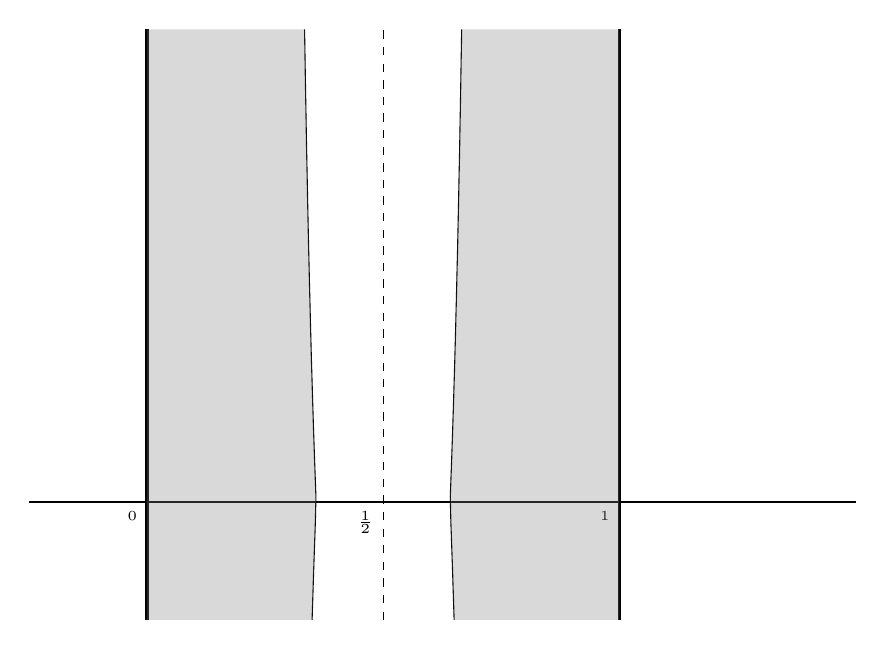
\begin{tikzpicture}[scale=3]
          \def\xmin{-0.5} \def\xmax{3}
          \def\ymin{-0.5} \def\ymax{2}
          \draw[thick] (\xmin,0) -- (\xmax,0);
          \draw[very thick] (0,\ymin) -- (0,\ymax);
          \draw[very thick] (2,\ymin) -- (2,\ymax);
          \draw[dashed] (1,\ymin) -- (1,\ymax);

          \node at (0,0) [below left] {\tiny{$0$}};
          \node at (1,0) [below left] {\tiny{$\frac{1}{2}$}};
          \node at (2,0) [below left] {\tiny{$1$}};

          \draw[domain=-0.5:2,variable=\y] plot({1.5-((0.3)/ln(4+abs(\y)))},\y);
          \draw[domain=-0.5:2,variable=\y] plot({0.5+((0.3)/ln(4+abs(\y)))},\y);

          \fill [gray,opacity=0.3,domain=-0.5:2,variable=\y]
          (1.5, 2)
          -- (2,2) 
          -- (2,-0.5)
          -- (1.5,-0.5)
          -- plot({1.5-((0.3)/ln(4+abs(\y)))},\y)
          -- cycle;

          \fill [gray,opacity=0.3,domain=-0.5:2,variable=\y]
          (0.5, 2)
          -- (0,2) 
          -- (0,-0.5)
          -- (0,-0.5)
          -- plot({0.5+((0.3)/ln(4+abs(\y)))},\y)
          -- cycle;
          \end{tikzpicture}
        \caption{The classical zero-free region for $\z(s)$ (symmetrized).}
        \label{fig:classical_zero-free_region}
      \end{figure}

      A couple of comments are in order. The classical zero-free region describes a zero-free region for the Riemann zeta function in the right-half of the critical strip. As the zeros are symmetric about the critical line, we immediately obtain a zero-free region symmetric about the critical line (see \cref{fig:classical_zero-free_region}). This region has been improved many times. In 1922, the breadth of the zero-free region was enlarged to 
      \[
        \frac{c\log\log(|t|+2)}{\log(|t|+2)},
      \]
      by Littlewood, and in 1958 Vinogradov and Korobov independently enlarged the zero-free region to
      \[
        \frac{c}{(\log(|t|+2))^{\a}},
      \]
      for any $\a > \frac{2}{3}$ and where $c$ depends upon $\a$ (see \cite{davenport1980multiplicative} for a more detailed historical account). These improvements depend on upper bounds for $\z(s)$ is a region just to the left of $\Re(s) = 1$ and these upper bounds are deduced from delicate estimates of exponential sums. It is important to mention that the constant $c$ is in general different for all the zero-free regions. This means $c$ depends implicitly upon the shape of the zero-free region. Many current problems revolve around making improvements upon zero-free region results. Also, the constant $c$ is effective and there are constant efforts to compute it to high degrees of precision.

      It is also an interesting question to know the height of the first zero (with nonnegative imaginary part) the Riemann zeta function. It is not difficult to show that this height must necessarily be positive. In other words, $\z(s) \neq 0$ for $0 < s < 1$ (we know $\z(0) = -\frac{1}{2}$ and that there is a pole at $s = 1$). One way to see this is to consider the \textbf{Dirichlet eta function}\index{Dirichlet eta function} $\eta(s)$ defined by
      \[
        \eta(s) = \sum_{n \ge 1}\frac{(-1)^{n-1}}{n^{s}}.
      \]
      Note that $\eta(s)$ converges for $\Re(s) > 0$ by \cref{prop:Dirichlet_series_convergence_bounded_coefficient_sum}. Now for real $s$ with $0 < s < 1$ and even $n$, $\frac{1}{n^{s}}-\frac{1}{(n+1)^{s}} > 0$ so that $\eta(s) > 0$. But for $\Re(s) > 0$, we have
      \[
        (1-2^{1-s})\z(s) = \sum_{n \ge 1}\frac{1}{n^{s}}-2\sum_{n \ge 1}\frac{1}{(2n)^{s}} = \sum_{n \ge 1}\frac{(-1)^{n-1}}{n^{s}} = \eta(s).
      \]
      Therefore $\z(s)$ cannot admit a zero for $0 < s < 1$ because then $\eta(s)$ would be zero too. Actually, since $1-2^{1-s} < 0$ in this segment we also know $\z(s) < 0$ in this segment as well. As for the height of the first zero, it occurs on the critical line (as predicted by the Riemann hypothesis) at height $t \approx 14.134$. In particular, this gives a slight improvement to the classical zero-free region in \cref{fig:classical_zero-free_region}. Actually, the first $15$ zeros were computed by Gram in 1903 (see \cite{gram1903note}). Since then, billions of zeros have been computed and have all been verified to lie on the critical line.
    \subsection*{The Classical Zero-free Region for \texorpdfstring{$L(s,\chi)$}{L(s,\chi)} \& Siegel Zeros}
      For a fixed Dirichlet character $\chi$ of conductor $q$, it is not difficult to obtain a zero-free region result for $L(s,\chi)$ analogous to the classical zero-free region for $\z(s)$. However, it is more useful to have zero-free regions in terms of $q$ alone so that the character $\chi$ can vary. Unfortunately, an additional obstruction arises in the case that the character is quadratic. This is due to the possible existance of an additional real zero. Throughout, we will only be interested in non-principal characters. For convenience we use the standard notation
      \[
        \mathscr{L} = \log(q(|t|+2)),
      \]
      because this quantity appears all too often. The classical result, analogous to the case for the Riemann zeta function, is the following:

      \begin{theorem}[The classical zero-free region for $L(s,\chi)$]
        There exists a positive constant $c$ such that for any non-principal Dirichlet character $\chi$ of conductor $q > 1$, $L(s,\chi)$ contains no zeros in the region
        \[
          \left\{s = \s+it \in \C:\s > 1-\frac{c}{\scL}\right\},
        \]
        unless $\chi$ is quadratic in which case $L(s,\chi)$ has at most one, necessarily real, zero in this region.
      \end{theorem}
      \begin{proof}[Proof of the classical zero-free region for $L(s,\chi)$]
        We will eventually break the argument depending on whether $\chi$ is quadratic or complex, but for the moment we only assume $\chi$ is primitive. Let $s = \s+it$ and suppose $1 < \s \le 2$. We will derive bounds for each of the terms in \cref{lem:zero-free_region_Dirichlet_lemma}. For the first term, since $L(s,\chi_{q,0})$ has a simple pole at $s = 1$, $-\frac{L'}{L}(s,\chi_{q,0})$ has a simple pole there too. Therefore
        \begin{equation}\label{equ:classical_zero-free_region_Dirichlet_1}
          -\frac{L'}{L}(\s,\chi_{q,0}) < A+\frac{1}{\s-1},
        \end{equation}
        for some positive constant $A$. For the middle term, $\frac{s+\mf{a}}{2} \sim |t|+2$ so by \cref{equ:approximtion_for_digamma}, $\frac{\G'}{\G}\left(\frac{s+\mf{a}}{2}\right) = \log(|t|+2)+O(1) = O(\log(|t|+2))$. This estimate and explicit formula for $\frac{L'}{L}(s,\chi)$ together give
        \begin{equation}\label{equ:classical_zero-free_region_Dirichlet_2}
          -\Re\left(\frac{L'}{L}(s,\chi)\right) < A\scL-\Re(B(\chi))-\sum_{\rho}\Re\left(\frac{1}{s-\rho}+\frac{1}{\rho}\right),
        \end{equation}
        where we take $A$ larger (to satisfy the $O$-estimate) if necessary. Upon substituting \cref{equ:B_chi_computation_3} into \cref{equ:classical_zero-free_region_Dirichlet_2} we obtain the simpler expression
        \begin{equation}\label{equ:classical_zero-free_region_Dirichlet_3}
          -\Re\left(\frac{L'}{L}(s,\chi)\right) < A\scL-\sum_{\rho}\Re\left(\frac{1}{s-\rho}\right).
        \end{equation}
        If $\rho = \b+i\g$, $\Re\left(\frac{1}{s-\rho}\right) = \frac{\s-\b}{(\s-\b)^{2}+(t+\g)^{2}} \ge 0$ which implies the sum in \cref{equ:classical_zero-free_region_Dirichlet_3} is a sum of nonnegative terms and hence any part of it may be discarded. Now suppose $\chi$ is primitive and complex. We claim that \cref{equ:classical_zero-free_region_Dirichlet_3} holds for $L(s,\chi^{2})$ too for a possibly larger constant $A$. This is certainly true if $\chi^{2}$ is primitive, but when $\chi^{2}$ is not primitive we have a minor complication. To get around this complication, let $\wtilde{\chi}$ be the primitive character inducing $\chi^{2}$. Taking the logarithmic derivative of \cref{equ:non-primitive_primitive_Dirichlet_L-series_relation} with $\chi^{2}$ in place of $\chi$, we find that
        \begin{equation}\label{equ:classical_zero-free_region_Dirichlet_4}
          \left|\frac{L'}{L}(s,\chi^{2})-\frac{L'}{L}(s,\wtilde{\chi})\right| = \left|\sum_{p \mid q}\frac{\wtilde{\chi}(p)\log(p)p^{-s}}{1-\wtilde{\chi}(p)p^{-s}}\right| \le \sum_{p \mid q}\frac{\log(p)p^{-\s}}{1-p^{-\s}} \le \sum_{p \mid q}\log(p) \le \log(q).
        \end{equation}
        Now \cref{equ:classical_zero-free_region_Dirichlet_4} implies the weaker inequality
        \begin{equation}\label{equ:classical_zero-free_region_Dirichlet_5}
          -\Re\left(\frac{L'}{L}(s,\chi^{2})\right) \le \log(q)-\Re\left(\frac{L'}{L}(s,\wtilde{\chi})\right),
        \end{equation}
        and combining \cref{equ:classical_zero-free_region_Dirichlet_3,equ:classical_zero-free_region_Dirichlet_5} with $\wtilde{\chi}$ in place of $\chi$ yields
        \begin{equation}\label{equ:classical_zero-free_region_Dirichlet_6}
            -\Re\left(\frac{L'}{L}(s,\chi^{2})\right) < A\scL-\sum_{\rho}\Re\left(\frac{1}{s-\rho}\right),
        \end{equation}
        for a possibly larger constant $A$. We can now obtain the bound on the last term. Taking $s = \s+2it$ and discarding the entire sum, \cref{equ:classical_zero-free_region_Dirichlet_6} gives
        \begin{equation}\label{equ:classical_zero-free_region_Dirichlet_7}
          -\Re\left(\frac{L'}{L}(s+2it,\chi)\right) < A\scL,
        \end{equation}
        for a possibly larger constant $A$. For the middle term, assume $t = \g$ is the ordinate of the zero $\rho = \b+i\g$. Letting $s = \s+it$ and retaining only the term in the sum corresponding to $\rho$, \cref{equ:classical_zero-free_region_Dirichlet_3} implies
        \begin{equation}\label{equ:classical_zero-free_region_Dirichlet_8}
            -\Re\left(\frac{L'}{L}(\s+it,\chi^{2})\right) < A\scL-\frac{1}{\s-\b}.
        \end{equation}
        Upon combining \cref{equ:classical_zero-free_region_Dirichlet_1,equ:classical_zero-free_region_Dirichlet_7,equ:classical_zero-free_region_Dirichlet_8} with \cref{lem:zero-free_region_Dirichlet_lemma} we obtain
        \[
          0 < 3A+\frac{3}{\s-1}+5A\scL-\frac{4}{\s-\b},
        \]
        which, taking $A$ to be larger if necessary, gives
        \begin{equation}\label{equ:zero-free_region_estimate_Dirichlet_9}
          0 < \frac{3}{\s-1}+5A\scL-\frac{4}{\s-\b}.
        \end{equation}
        Letting $\d$ be such that $\s = 1+\frac{\d}{\scL}$, \cref{equ:zero-free_region_estimate_Dirichlet_9} becomes
        \[
          0 < \left(5A+\frac{3}{\d}\right)\scL-\frac{4}{(1-\b)+\frac{\d}{\scL}}.
        \]
        Arguing exactly as in the proof of the classical zero-free region for $\z(s)$, we obtain a bound of the form
        \begin{equation}\label{equ:zero-free_region_estimate_Dirichlet_beta_bound}
          \b < 1-\frac{c}{\scL}.
        \end{equation}
        It follows that there can be no zero in the region
        \begin{equation}\label{equ:zero-free_region_estimate_Dirichlet_sigma_bound}
          \s \ge 1-\frac{c}{\scL},
        \end{equation}
        for all $\s$ and $t$. This finishes the proof in the case that $\chi$ is primitive and complex. Actually, the assumption that $\chi$ is primitive can be dropped since if $\wtilde{\chi}$ induces $\chi$ then \cref{equ:non-primitive_primitive_Dirichlet_L-series_relation} implies that any zero of $L(s,\chi)$ which is not a zero of $L(s,\wtilde{\chi})$ is a zero of one of the factors $(1-\wtilde{\chi}(p)p^{-s})$ and hence lies on the line $\Re(s) = 0$ which is a boundary line of the critial strip. Therefore our zero-free region holds for all complex $\chi$. We now suppose $\chi$ is primitive and quadratic. The only part of the argument that needs adjustment is upper bound for the last term. \cref{equ:classical_zero-free_region_Dirichlet_4,equ:classical_zero-free_region_Dirichlet_5} still hold but since $\chi^{2} = \chi_{q,0}$, the primitive character inducing $\chi^{2}$ is the trivial character so $L(s,\wtilde{\chi}) = \z(s)$ and hence \cref{equ:classical_zero-free_region_Dirichlet_3} with $\wtilde{\chi}$ in place of $\chi$ no longer applies. Instead, we use the explicit formula for $\frac{\z'}{\z}(s)$. Since $\frac{s}{2}+1 \sim |t|+2$, \cref{equ:approximtion_for_digamma} implies $\frac{\G'}{\G}\left(\frac{s}{2}+1\right) = \log(|t|+2)+O(1) = O(\log(|t|+2))$. This estimate, the explicit formula for $\frac{\z'}{\z}(s)$, and discarding the sum over nontrivial zeros (because this is a sum of nonpositive terms), together give
        \begin{equation}\label{equ:classical_zero-free_region_Dirichlet_10}
          -\Re\left(\frac{\z'}{\z}(s)\right) < \Re\left(\frac{1}{s-1}\right)+A\log(|t|+2),
        \end{equation}
        for some possibly larger constant $A$. Observe that the term corresponding to $\frac{1}{s-1}$ in the explicit formula for $\frac{\z'}{\z}(s)$ is present in \cref{equ:classical_zero-free_region_Dirichlet_10} because $t$ may very well be small and so this term is not necessarily bounded from above. Letting $s = \s+2it$, and combining \cref{equ:classical_zero-free_region_Dirichlet_5,equ:classical_zero-free_region_Dirichlet_10} (recall $L(s,\wtilde{\chi}) = \z(s)$) yields
        \begin{equation}\label{equ:classical_zero-free_region_Dirichlet_11}
          -\Re\left(\frac{L'}{L}(\s+2it,\chi^{2})\right) < \Re\left(\frac{1}{\s-1+2it}\right)+A\scL,
        \end{equation}
        for some possibly larger constant $A$. Combining \cref{equ:classical_zero-free_region_Dirichlet_1,equ:classical_zero-free_region_Dirichlet_7,equ:classical_zero-free_region_Dirichlet_11} with \cref{lem:zero-free_region_Dirichlet_lemma} gives
        \[
          0 < 3A+\frac{3}{\s-1}+5A\scL+\Re\left(\frac{1}{\s-1+2it}\right)-\frac{4}{\s-\b},
        \]
        and taking $A$ to be larger if necessary, we have
        \begin{equation}\label{equ:classical_zero-free_region_Dirichlet_12}
          0 < \frac{3}{\s-1}+5A\scL+\Re\left(\frac{1}{\s-1+2it}\right)-\frac{4}{\s-\b}.
        \end{equation}
        Let $\d$ be such that $\s = 1+\frac{\d}{\scL}$. If we also assume $|t| \ge \frac{\d}{\scL}$, then $\Re\left(\frac{1}{\s-1+2it}\right) = \frac{\s-1}{(\s-1)^{2}+2t^{2}} \le \frac{1}{5\d}\scL$ and \cref{equ:classical_zero-free_region_Dirichlet_12} becomes
        \[
          0 < \left(5A+\frac{3}{\d}+\frac{1}{5\d}\right)\scL-\frac{4}{(1-\b)+\frac{\d}{\log|t|}}.
        \]
        The additional estimate $|t| \ge \frac{\d}{\scL}$ is essential, because if $t$ is close to $0$ and $\s$ is close to $1$, then $\Re\left(\frac{1}{\s-1+2it}\right)$ is not bounded from above. Arguing again as in the proof of the classical zero-free region for $\z(s)$, we arrive at the bound \cref{equ:zero-free_region_estimate_Dirichlet_beta_bound} for some possibly larger constant $c$. Therefore \cref{equ:zero-free_region_estimate_Dirichlet_sigma_bound} holds for primitive quadratic $\chi$. Just as for complex characters, we can remove the primitive assumption by appealing \cref{equ:non-primitive_primitive_Dirichlet_L-series_relation}. So altogether, we have the desired zero-free region for all complex characters for all $t$ and all quadratic characters with $|t| \ge \frac{\d}{\scL}$ for some $\d$. It remains to show that in the quadratic case, that there is at most one zero with $|t| < \frac{\d}{\scL}$ and that this zero is real. Actually it suffices to prove that there is at most one zero because if $\rho$ is a zero then so is $\conj{\rho}$ since $\chi$ is quadratic. But both $\rho$ and $\conj{\rho}$ have the same imaginary part in absolute value (so they both belong to this region). Again, we may assume $\chi$ is primitive. Now suppose there were two complex conjugate zeros $\rho = \b+i\g$ and $\conj{\rho} = \b-i\g$ belonging to the region $|t| < \frac{\d}{\scL}$. Taking $s = \s > 1$ in \cref{equ:classical_zero-free_region_Dirichlet_3} and retaining only the terms in the sum corresponding to these zeros, we have
        \begin{equation}\label{equ:classical_zero-free_region_Dirichlet_13}
          -\Re\left(\frac{L'}{L}(\s,\chi)\right) < A\scL-\frac{2(\s-\b)}{(\s-\b)^{2}+\g^{2}},
        \end{equation}
        where we have used $\Re\left(\frac{1}{\s-\rho}\right) = \frac{\s-\b}{(\s-\b)^{2}+\g^{2}}$. Appealing to \cref{equ:classical_zero-free_region_zeta_1,equ:Drichlet_series_log_derivative_zeta,equ:Drichlet_series_log_derivative_Dirichlet} we have the following crude lower bound:
        \begin{equation}\label{equ:classical_zero-free_region_Dirichlet_14}
          -\Re\left(\frac{L'}{L}(\s,\chi)\right) \ge \Re\left(\sum_{n \ge 1}\frac{\chi(n)\L(n)}{n^{\s}}\right) \ge \sum_{n \ge 1}\frac{\L(n)}{n^{\s}} = \frac{\z'}{\z}(\s) > -\frac{1}{\s-1}-A,
        \end{equation}
        for a possibly larger constant $A$. Taking $A$ larger, if necessary, \cref{equ:classical_zero-free_region_Dirichlet_13,equ:classical_zero-free_region_Dirichlet_14} together yield
        \begin{equation}\label{equ:classical_zero-free_region_Dirichlet_15}
          -\frac{1}{\s-1} < A\scL-\frac{2(\s-\b)}{(\s-\b)^{2}+\g^{2}}.
        \end{equation}
        Now let $\d$ (possibly a different $\d$ than before) be such that $\s = 1+\frac{\d}{\scL}$. Since $|\g| < \frac{\d}{\scL}$ by assumption, we have
        \[
          |\g| < \frac{\s-1}{2} < \frac{\s-\b}{2}.
        \]
        The estimate above implies $\g^{2} < \frac{(\s-\b)^{2}}{4}$ and inserting this into \cref{equ:classical_zero-free_region_Dirichlet_15} gives
        \[
          -\frac{1}{\s-1} < A\scL-\frac{5}{8(\s-\b)}.
        \]
        Upon solving for $\b$ and substiuting $\s = 1+\frac{\d}{\scL}$, we find that
        \[
          \b < 1+\frac{2\d-\frac{5}{8}\left(\frac{1}{2\d}+A\right)}{\scL}.
        \]
        Choosing $\d$ such that $2\d-\frac{5}{8}\left(\frac{1}{2\d}+A\right) < -1$ ($\d$ is free to choose because $\s$ is) results in the bound
        \[
          \b < 1-\frac{\d}{\scL},
        \]
        which contradicts the zero-free region just establish because $|\g| < \frac{\d}{\scL}$. Hence there cannot be two complex conjugate zeros. In the case of two real zeros $\rho = \b$ and $\rho' = \b'$, without loss of generality we may assume $\rho$ is such that $\Re\left(\frac{1}{s-\rho}\right) \le \Re\left(\frac{1}{s-\rho'}\right)$. Then taking $s = \s > 1$ in \cref{equ:classical_zero-free_region_Dirichlet_3} and only retaining the terms in the sum correspond to these zeros but bounding both of them by the term corresponding to $\rho$ gives \cref{equ:classical_zero-free_region_Dirichlet_13} and we may repeat the argument. In the case of a real zero $\rho = \b$ with multiplicity at least two, we perform the same procedure but only retain two terms in the sum corresponding to $\rho$ (because we at least have a double zero) and obtain \cref{equ:classical_zero-free_region_Dirichlet_13} with $\g = 0$. The same argument now works but is even simpler because we do not need to estimate $\g$. All of this shows that if there is a zero it must be a single real zero.
      \end{proof}

      The classical zero-free region for Dirichlet $L$-functions is almost an exact analog to the classical zero-free region for the Riemann zeta function. In particular, the constant $c$ is effective. The strength of this zero-free region result rests in the fact that it only depends upon the conductor $q$ of the character. Unfortunately, the drawback is that when $\chi$ is quadratic there may very well be a single real zero. Of course, the Selberg class Riemann hypothesis implies that such zeros do not exist. These hypothetical zeros are referred to as \textbf{Siegel zeros}\index{Siegel zeros} or \textbf{exceptional zeros}\index{exceptional zeros}. So far, no Siegel zero has been shown to exist or not exist. Now the effective constant $c$ is absolute and hence is independent of every quadratic character $\chi$. So for any fixed modulus, we can choose a smaller constant to make the region zero-free for all characters of that modulus. Also, some progress has been made towards showing that they are exceptionally rare (see \cite{montgomery2006multiplicative}):

      \begin{proposition}\label{prop:at_most_one_Siegel_zero_per_modulus}
        For every integer $q > 1$, there is at most one primitive and quadratic Dirichlet character $\chi$ of conductor $q$ such that $L(s,\chi)$ has a Siegel zero.
      \end{proposition}

      A natural question to ask after \cref{prop:at_most_one_Siegel_zero_per_modulus} is the following: how small can the distance between the moduli of two quadratic characters whose Dirichlet $L$-functions posess Siegel zeros be? This has been answered (see \cite{montgomery2006multiplicative} for a proof):

      \begin{proposition}\label{prop:modulus_distance_Siegel_zeros}
        For any positive $A > 0$ there exists a positive constant $c_{A}$ such that if $(q_{i})_{1 \le i \le n}$ is a strictly increasing sequence of positive integers with $q_{1} > 1$ and such that there exist primitive quadratic Dirichlet characters $\chi_{i}$ of conductor $q_{i}$ whose Dirichlet $L$-function $L(s,\chi_{q_{i}})$ posses Siegel zeros $\b_{i}$ such that
        \[
          \b_{i} > 1-\frac{c_{A}}{\log(q_{i})},
        \]
        for $1 \le i \le n$, then
        \[
          q_{i+1} > q_{i}^{A},
        \]
        for $1 \le i \le n-1$.
      \end{proposition}
    \subsection*{Siegel's Theorem}
      Siegel zeros present an unfortunate obstruction to zero-free region results for Dirichlet $L$-functions when the character $\chi$ is quadratic. However, if we no longer require the constant $c$ in the zero-free region to be effective, we can obtain a much better result for how close the Siegel zero can be to $1$. Ultimately, this improved bound results from a lower bound for $L(1,\chi)$ (recall that this is nonzero from our discussion of non-vanishing on $\Re(s) = 1$ ). \textbf{Siegel's theorem}\index{Siegel's theorem} refers to either this lower bound or to the improved zero-free region. In its first version, Siegel's theorem is the following:

      \begin{theorem}[Siegel's theorem, first version]
        Let $\chi$ be a primitive quadratic Dirichlet character modulo $q$. Then for any $\e > 0$ there exists a positive constant $c_{1}(\e)$ such that
        \[
          L(1,\chi) \ge c_{1}(\e)q^{-\e}.
        \]
      \end{theorem}

      In its second version, the statement is about how close a Siegel zero can be to $1$:

      \begin{theorem}[Siegel's theorem, second version]
        Let $\chi$ be a primitive quadratic Dirichlet character modulo $q$. Then for any $\e > 0$ there exists a positive constant $c_{2}(\e)$ such that $L(s,\chi)$ has no real zero $\b$ with
        \[
          1-\b \le c_{2}(\e)q^{-\e}.
        \]
      \end{theorem}

      The largest defect of Siegel's theorem, in either version, is that the implicit constants $c_{1}(\e)$ and $c_{2}(\e)$ are ineffective (and not necessarily equal). Actually, the first version is slighly stronger as it implies the second. We will prove the second version (given the first) first and then we will prove the first version. Before we begin, however, we need two small lemmas about the size of $L'(\s,\chi)$ and $L(\s,\chi)$ for real $s$ close to $1$:

      \begin{lemma}\label{lem:Siegels_theorem_second_version_lemma}
        Let $\chi$ be a Dirichlet character modulo $m > 1$. Then $L'(\s,\chi) = O(\log^{2}(m))$ for any $\s$ such that $0 \le 1-\s \le \frac{1}{\log(m)}$.
      \end{lemma}
      \begin{proof}
        Setting $A(X) = \sum_{n \le X}\chi(n)$ we have $A(X) \ll 1$ by \cref{cor:Dirichlet_orthogonality_relations} (i) and that $\chi$ is periodic. Therefore $\s_{c} \le 0$ by \cref{prop:Dirichlet_series_convergence_bounded_coefficient_sum}. Hence for $\s$ in the prescribed region, $L(\s,\chi)$ is holomorphic and its derivative is given by
        \[
          L'(\s,\chi) = \sum_{n \ge 1}\frac{\chi(n)\log(n)}{n^{\s}} = \sum_{n < m}\frac{\chi(n)\log(n)}{n^{\s}}+\sum_{n \ge m}\frac{\chi(n)\log(n)}{n^{\s}}.
        \]
        We will show that the last two sums are both $O(\log^{2}(m))$. For the first sum, if $n < m$, we have
        \[
          \left|\frac{\chi(n)\log(n)}{n^{\s}}\right| \le \frac{1}{n^{\s}}\log(n) = \frac{n^{1-\s}}{n}\log(n) < \frac{m^{1-\s}}{n}\log(n) < \frac{e}{n}\log(m),
        \]
        where the last inequality follows because $1-\s \le \frac{1}{\log(m)}$. Then
        \[
          \left|\sum_{n \le m}\frac{\chi(n)\log(n)}{n^{s}}\right| < e\log(m)\sum_{n < m}\frac{1}{n} < e\log(m)\int_{1}^{m}\frac{1}{n}\,dn \ll \log^{2}(m).
        \]
        For the second sum, $A(Y) \ll 1$ so that $A(Y)\log(Y)Y^{-\s} \to 0$ as $Y \to \infty$. Then Abel's summation formula (see \cref{append:Summation_Formulas}) gives
        \begin{equation}\label{equ:Siegels_theorem_second_version_lemma_1}
          \sum_{n \ge m}\frac{\chi(n)\log(n)}{n^{\s}} = -A(m)\log(m)m^{-\s}-\int_{m}^{\infty}A(u)(1-\s\log(u))u^{-(\s+1)}\,du.
        \end{equation}
        Since $0 \le 1-\s \le \frac{1}{\log(m)}$, we have $1-\s\log(u) \le \frac{\log(u)}{\log(m)}$. Also, we have the more precise estimate $|A(X)| \le m$ because $\chi$ is $m$-periodic and $|\chi(n)|$ is at most $1$. With these estimates and \cref{equ:Siegels_theorem_second_version_lemma_1} we make the following computation:
        \begin{align*}
          \left|\sum_{n \ge m}\frac{\chi(n)\log(n)}{n^{\s}}\right| &\le |A(m)|\log(m)m^{-\s}+\int_{m}^{\infty}|A(u)|(1-\s\log(u))u^{-(\s+1)}\,du \\
          &\le |A(m)|\log(m)m^{-\s}+\log(m)\int_{m}^{\infty}|A(u)|\log(u)u^{-(\s+1)}\,du \\
          &\le m^{1-\s}\log(m)+m\int_{m}^{\infty}\log(u)u^{-(\s+1)}\,du \\
          &= m^{1-\s}\log(m)+m\left(-\log(u)\frac{u^{-\s}}{\s}\bigg|_{m}^{\infty}+\int_{m}^{\infty}\frac{u^{-(\s+1)}}{s}\,du\right) \\
          &= m^{1-\s}\log(m)+m\left(-\log(u)\frac{u^{-\s}}{\s}-\frac{u^{-\s}}{\s^{2}}\right)\bigg|_{m}^{\infty} \\
          &= m^{1-\s}\log(m)+m\left(\log(m)\frac{m^{-\s}}{\s}+\frac{m^{-\s}}{\s^{2}}\right) \\
          &\ll m^{1-\s}\log(m) \\
          &\ll e\log(m),
        \end{align*}
        where in the fourth line we have used integration by parts and the last line holds because $1-\s \le \frac{1}{\log(m)}$. But $e\log(m) = O(\log^{2}(m))$ so the second sum is also $O(\log^{2}(m))$. Therefore we have shown $L'(\s,\chi) = O(\log^{2}(m))$ finishing the proof. 
      \end{proof}

      The second lemma is even easier and is proved in exactly the same way:

      \begin{lemma}\label{lem:Siegels_theorem_first_version_lemma}
        Let $\chi$ be a Dirichlet character modulo $m > 1$. Then $L(\s,\chi) = O(\log(m))$ for any $\s$ such that $0 \le 1-\s \le \frac{1}{\log(m)}$.
      \end{lemma}
      \begin{proof}
        Note that
        \[
          L(\s,\chi) = \sum_{n \ge 1}\frac{\chi(n)}{n^{\s}} = \sum_{n < m}\frac{\chi(n)}{n^{\s}}+\sum_{n \ge m}\frac{\chi(n)}{n^{\s}}.
        \]
        It suffices to show that the last two sums are both $O(\log^{2}(m))$. For the first sum, since $n < m$, we have
        \[
          \left|\frac{\chi(n)}{n^{\s}}\right| \le \frac{1}{n^{\s}} = \frac{n^{1-\s}}{n} < \frac{m^{1-\s}}{n} < \frac{e}{n},
        \]
        where the last inequality follows because $1-\s \le \frac{1}{\log(m)}$. Therefore
        \[
          \left|\sum_{n \le m}\frac{\chi(n)}{n^{s}}\right| < e\sum_{n < m}\frac{1}{n} < e\log(m)\int_{1}^{m}\frac{1}{n}\,dn \ll \log(m).
        \]
        As for the second sum, setting $A(Y) = \sum_{n \le Y}\chi(n)$ we have $A(Y) \ll 1$ so that $A(Y)Y^{-\s} \to 0$ as $Y \to \infty$. Then Abel's summation formula (see \cref{append:Summation_Formulas}) gives
        \begin{equation}\label{equ:Siegels_theorem_first_version_lemma_1}
          \sum_{n \ge m}\frac{\chi(n)}{n^{\s}} = -A(m)m^{-\s}-\int_{m}^{\infty}A(u)u^{-(\s+1)}\,du.
        \end{equation}
        Using the more precise estimate $|A(X)| \le m$ because $\chi$ is $m$-periodic and $|\chi(n)|$ is at most $1$ and \cref{equ:Siegels_theorem_first_version_lemma_1}, we make the following computation:
        \begin{align*}
          \left|\sum_{n \ge m}\frac{\chi(n)\log(n)}{n^{\s}}\right| &\le |A(m)|m^{-\s}+\int_{m}^{\infty}|A(u)|u^{-(\s+1)}\,du \\
          &\le |A(m)|m^{-\s}+\int_{m}^{\infty}|A(u)|\log(u)u^{-(\s+1)}\,du \\
          &\le m^{1-\s}+m\int_{m}^{\infty}\log(u)u^{-(\s+1)}\,du \\
          &= m^{1-\s}+m\left(-\log(u)\frac{u^{-\s}}{\s}\bigg|_{m}^{\infty}+\int_{m}^{\infty}\frac{u^{-(\s+1)}}{s}\,du\right) \\
          &= m^{1-\s}+m\left(-\log(u)\frac{u^{-\s}}{\s}-\frac{u^{-\s}}{\s^{2}}\right)\bigg|_{m}^{\infty} \\
          &= m^{1-\s}+m\left(\log(m)\frac{m^{-\s}}{\s}+\frac{m^{-\s}}{\s^{2}}\right) \\
          &\ll m^{1-\s} \\
          &\ll e,
        \end{align*}
        where in the fourth line we have used integration by parts and the last line holds because $1-\s \le \frac{1}{\log(m)}$. But $e = O(\log^{2}(m))$ so the second sum is also $O(\log^{2}(m))$. Therefore we have shown $L(\s,\chi) = O(\log(m))$ which completes the proof.
      \end{proof}

      We will now prove the second version of Sigel's theorem, assuming the first, and using \cref{lem:Siegels_theorem_second_version_lemma}:

      \begin{proof}[Proof of Siegel's theorem, second version]
        We we will prove the theorem by contradiction. Let $\e > 0$. Clearly the result holds for a single $q$, and notice that the result also holds provided we bound $q$ from above by taking the maximum of all the $c_{2}(\e)$. Therefore we may suppose $q$ is arbitrarily large. In this case, if there was a real zero $\b$ with $1-\b \le c_{2}(\e)q^{-\e}$ then for large enough $q$ we have $0 \le 1-\b \le \frac{1}{\log(q)}$ so that $L'(\s,\chi) = O(\log^{2}(q))$ for $\b \le \s \le 1$ by \cref{lem:Siegels_theorem_second_version_lemma}. These two estimates and the mean value theorem together give
        \[
          L(1,\chi) = L(1,\chi)-L(\b,\chi) = L'(\s,\chi)(1-\b) \ll \log^{2}(q)q^{-\e}.
        \]
        Upon taking $\frac{\e}{2}$ in the first version of Siegel's theorem, we obtain
        \[
          q^{-\frac{\e}{2}} \ll L(1,\chi) \ll \log^{2}(q)q^{-\e},
        \]
        which is a contradiction for large $q$.
      \end{proof}

      It remains to prove the first version of Siegel's theorem. The idea is to combine two Dirichlet $L$-functions attached to distinct characters with distinct moduli and use this new $L$-function to derivative a lower bound for a single Dirichlet $L$-function at $s = 1$:

      \begin{proof}[Proof of Siegel's theorem, first version]
        Let $\chi_{1}$ and $\chi_{2}$ be two primitive quadratic and non-principal characters modulo $q_{1}$ and $q_{2}$ repsectively. Set
        \[
          F(s) = \z(s)L(s,\chi_{1})L(s,\chi_{2})L(s,\chi_{1}\chi_{2}).
        \]
        The key ingredient in the proof is a lower bound for $F(s)$ relative to the modulus $q_{1}q_{2}$ in a small interval on the real axis close to $1$. We will first deduce this estiamte from which the rest of the proof follows easily. Observe that $F(s)$ is holomorphic on $\C$ except for a simple pole at $s = 1$. Let $\l$ be the residue at this pole so that
        \[
          \l = L(1,\chi_{1})L(1,\chi_{2})L(1,\chi_{1}\chi_{2}).
        \]
        Taking the logarithim of $F(s)$ with $\Re(s) > 1$ and using \cref{equ:log_Dirichlet_L-function_expansion} gives
        \[
          \log F(s) = \sum_{p}\sum_{k \ge 1}\frac{1+\chi_{1}(p^{k})+\chi_{2}(p^{k})+(\chi_{1}\chi_{2})(p^{k})}{kp^{ks}} = \sum_{p}\sum_{k \ge 1}\frac{(1+\chi_{1}(p^{k}))(1+\chi_{2}(p^{k}))}{kp^{ks}}.
        \]
        Since $(1+\chi_{1}(p^{k}))(1+\chi_{2}(p^{k}))$ is nonnegative, the coefficients of $\log F(s)$ are nonnegative and therefore the coefficients of $F(s)$, call them $a(n)$, are nonnegative as well. Moreover, $a(0) = 1$ which can be seen by expanding out the Dirichlet series defining $F(s)$. Now $F(s)$ is represented as an absolutely convergent series for $\Re(s) > 1$ so that it has a power series expansion about $s = 2$ with radius $1$:
        \[
          F(s) = \sum_{m \ge 0}\frac{F^{(m)}(2)}{m!}(s-2)^{m},
        \]
        for $|s-2| < 1$. We can compute $F^{(m)}(2)$ using the Dirichlet series by differentiating termwise:
        \begin{equation}\label{equ:Siegels_theorem_first_version_1}
          F^{(m)}(2) = \frac{d^{m}}{ds^{m}}\left(\sum_{n \ge 1}\frac{a(n)}{n^{s}}\right)\Bigg|_{s = 2} = (-1)^{m}\sum_{n \ge 1}\frac{a(n)\log^{m}(n)}{n^{s}}\Bigg|_{s = 2} = (-1)^{m}\sum_{n \ge 1}\frac{a(n)\log^{m}(n)}{n^{2}}.
        \end{equation}
        Since the $a(n)$ are nonnegative, as just mentioned, it follows that $F^{(m)}(2)$ is nonnegative and therefore we may write
        \[
          F(s) = \sum_{m \ge 0}b(m)(2-s)^{m},
        \]
        for $|s-2| < 1$ and with $b(m)$ nonnegative. Also, \cref{equ:Siegels_theorem_first_version_1} and the fact that the $a(n)$ are nonnegative with $a(0) = 1$ together imply that $b(0) > 1$. Then
        \begin{equation}\label{equ:Siegels_theorem_first_version_2}
          F(s)-\frac{\l}{s-1} = F(s)-\l\sum_{m \ge 0}(2-s)^{m} = \sum_{m \ge 0}(b(m)-\l)(2-s)^{m},
        \end{equation}
        and the last series must be absolutely convergent for say $|s-2| < 2$ because $F(s)-\frac{\l}{s-1}$ is entire as we have removed the pole at $s = 1$. We now wish to estiamte $F(s)$ and $\frac{\l}{s-1}$ on the circle $|s-2| = \frac{3}{2}$. Let $\chi$ be a Dirichlet character modulo $q$ and let $A(X) = \sum_{n \le X}\chi(n)$. Then Abel's summation formula and that $A(X) \ll 1$ (just as in the proof of \cref{prop:Dirichlet_series_convergence_bounded_coefficient_sum}) together imply
        \[
          L(s,\chi) = s\int_{1}^{\infty}A(u)u^{-(s+1)}\,du,
        \]
        for $\Re(s) > 0$. Restrict to $\Re(s) \ge \frac{1}{2}$ and let $s = \s+it$. As $|A(X)| \le q$, we obtain
        \[
          |L(s,\chi)| \le q|s|\int_{1}^{\infty}u^{-(\s+1)}\,du = -q|s|\frac{u^{-\s}}{\s}\bigg|_{1}^{\infty} = \frac{q|s|}{\s} \le 2q|s|.
        \]
        In particular, on the disk $|s-2| \le \frac{3}{2}$ we have the estimates
        \[
          |L(s,\chi_{1})| \ll q_{1}, \quad |L(s,\chi_{2})| \ll q_{2}, \quad \text{and} \quad |L(s,\chi_{1}\chi_{2})| \ll q_{1}q_{2}.
        \]
        Since $\z(s)$ is bounded on the circle $|s-2| = \frac{3}{2}$ (it's a compact set) and $\l = L(1,\chi_{1})L(1,\chi_{2})L(1,\chi_{1}\chi_{2})$, we obtain the bounds
        \[
          |F(s)| \ll q_{1}^{2}q_{2}^{2} \quad \text{and} \quad \left|\frac{\l}{s-1}\right| \ll q_{1}^{2}q_{2}^{2},
        \]
        on this circle as well. Cauchy's inequality for the size of coefficients of a power series applied to \cref{equ:Siegels_theorem_first_version_2} on the circle $|s-2| = \frac{3}{2}$ gives
        \begin{equation}\label{equ:Siegels_theorem_first_version_3}
          |b(m)-\l| \ll q_{1}^{2}q_{2}^{2}\left(\frac{2}{3}\right)^{m}.
        \end{equation}
        Let $M$ be a positive integer. For real $s$ with $\frac{7}{8} < s < 1$ we have $2-s < \frac{9}{8}$ and using \cref{equ:Siegels_theorem_first_version_2,equ:Siegels_theorem_first_version_3} together we can upper bound the tail of $F(s)-\frac{\l}{s-1}$:
        \begin{align*}
          \left|\sum_{m \ge M}(b(m)-\l)(2-s)^{m}\right| &\le \sum_{m \ge M}|b(m)-\l|(2-s)^{m} \\
          &\ll q_{1}^{2}q_{2}^{2}\sum_{m \ge M}\left(\frac{2}{3}(2-s)\right)^{m} \\
          &\ll q_{1}^{2}q_{2}^{2}\sum_{m \ge M}\left(\frac{3}{4}\right)^{m} \\
          &\ll q_{1}^{2}q_{2}^{2}\left(\frac{3}{4}\right)^{M} \\
          &\ll q_{1}^{2}q_{2}^{2}e^{-\frac{M}{4}},
        \end{align*}
        where the last estimate follows because $(\frac{3}{4})^{M} < e^{-\frac{M}{4}}$ (which is equivalent to $\log\left(\frac{3}{4}\right) < -\frac{1}{4}$). Let $c$ be the implict constant. Using that the $b(m)$ are nonnegative, $b(0) > 1$, and the previous estimate for the tail, we can estimate $F(s)-\frac{\l}{s-1}$ from below for $\frac{7}{8} < s < 1$. Ineed, throwing away the $b(m)$ terms for $1 \le m \le M$, bounding the constant term below by $1$, and use the tail estimate gives
        \begin{equation}\label{equ:Siegels_theorem_first_version_4}
          F(s)-\frac{\l}{s-1} \ge 1-\l\sum_{0 \le m \le M-1}(2-s)^{m}-cq_{1}^{2}q_{2}^{2}e^{-\frac{M}{4}} = 1-\l\frac{(2-s)^{M}-1}{1-s}-cq_{1}^{2}q_{2}^{2}e^{-\frac{M}{4}},
        \end{equation}
        which is valid for any positive integer $M$. Now chose $M$ to be a positive integer such that
        \begin{equation}\label{equ:Siegels_theorem_first_version_5}
          \frac{1}{2}e^{-\frac{1}{4}} \le cq_{1}^{2}q_{2}^{2}e^{-\frac{M}{4}} < \frac{1}{2}.
        \end{equation}
        Upon isolating $F(s)$ in \cref{equ:Siegels_theorem_first_version_4} and using the second estimate in \cref{equ:Siegels_theorem_first_version_5}, we get
        \begin{equation}\label{equ:Siegels_theorem_first_version_6}
          F(s) \ge \frac{1}{2}-\l\frac{(2-s)^{M}}{1-s}.
        \end{equation}
        Taking the logarithm of the first esimate in \cref{equ:Siegels_theorem_first_version_5} and isolating $M$, we obtain
        \begin{equation}\label{equ:Siegels_theorem_first_version_7}
          M \le 8\log(q_{1}q_{2})+c,
        \end{equation}
        for some different constant $c$. It follows that
        \begin{equation}\label{equ:Siegels_theorem_first_version_8}
          (2-s)^{M} = e^{M\log(2-s)} < e^{M(1-s)} \le c(q_{1}q_{2})^{8(1-s)},
        \end{equation}
        for some different constant $c$, where in the first estimate we have used the Taylor series of the logarithm truncated at the first term and in the second estimate we have used \cref{equ:Siegels_theorem_first_version_7}. Since $1-s$ is positive for $\frac{7}{8} < s < 1$, we can combine \cref{equ:Siegels_theorem_first_version_6,equ:Siegels_theorem_first_version_8} which gives
        \begin{equation}\label{equ:Siegels_theorem_first_version_9}
          F(s) \ge \frac{1}{2}-\l\frac{c}{1-s}(q_{1}q_{2})^{8(1-s)}.
        \end{equation}
        This is our desired lower bound for $F(s)$. Now let $\e > 0$ be given. We will choose the character $\chi_{1}$ depending upon $\e$. If there exists a Siegel zero $\b_{1}$ with $1-\frac{\e}{16} < \b_{1} < 1$, let $\chi_{1}$ be such a character correspoding to the Dirichlet $L$-function that admits this Siegel zero. Then $F(\b_{1}) = 0$ independent of the choice of $\chi_{2}$. If there is no such Siegel zero, choose $\chi_{1}$ to be any quadratic primitive character and $\b_{1}$ to be any number such that $1-\frac{\e}{16} < \b_{1} < 1$. Then $F(\b_{1}) < 0$ independent of the choice of $\chi_{2}$. Indeed, $\z(s)$ is negative in this segment (actually for $0 \le s < 1$) and each of the Dirichlet $L$-function defining $F(s)$ is positive at $s = 1$ (the Euler product implies Dirichlet $L$-function are positive for real $s > 1$ and they are in fact nonzero for $s = 1$ by \cref{thm:non-vanishing_of_Dirichlet_L-functions_at_s=1}) and do not admit a zero for $\b_{1} \le s \le 1$ by our choice of $\b_{1}$. In either case, $F(\b_{1}) \le 0$ so isolating $\l$ and disregarding the constants in \cref{equ:Siegels_theorem_first_version_9} with $s = \b_{1}$ gives the weaker estimate
        \begin{equation}\label{equ:Siegels_theorem_first_version_10}
          \l \gg (1-\b_{1})(q_{1}q_{2})^{-8(1-\b_{1})}.
        \end{equation}
        We will now choose $\chi_{2} = \chi$ and hence $q_{2} = q$ as in the statement of the theorem. Notice that, independent of any work we have done, the theorem holds for a single $q$. Moreover, the theorem holds provided we bound $q$ from above by taking the minimum of the $c_{1}(\e)$. Therefore we may assume $q$ is arbitrarily large and in particular that $q > q_{1}$. Using \cref{lem:Siegels_theorem_first_version_lemma} with $\s = 1$ applied to $L(s,\chi_{1})$ and $L(s,\chi_{1}\chi)$ and that Dirichlet $L$-function take positive real values at $s = 1$, we obtain
        \begin{equation}\label{equ:Siegels_theorem_first_version_11}
          \l \ll \log(q_{1})\log(q_{1}q)L(1,\chi).
        \end{equation}
        Combining \cref{equ:Siegels_theorem_first_version_10,equ:Siegels_theorem_first_version_11} yields
        \[
          (1-\b_{1})(q_{1}q)^{-8(1-\b_{1})} \ll \log(q_{1})\log(q_{1}q)L(1,\chi).
        \]
        As $\b_{1}$ and $q_{1}$ are fixed and $\log(q_{1}q) = O(\log(q))$, isolating $L(1,\chi)$ gives the weaker estimate
        \begin{equation}\label{equ:Siegels_theorem_first_version_12}
          L(1,\chi) \gg q^{-8(1-\b_{1})}(\log(q))^{-1}.
        \end{equation}
        But $1-\frac{\e}{16} < \b < 1$ so that $0 < 8(1-\b) < \frac{\e}{2}$ which combined with \cref{equ:Siegels_theorem_first_version_12} yields
        \[
          L(1,\chi) \gg q^{-\frac{\e}{2}}(\log(q))^{-1} \gg q^{-\e},
        \]
        where the last estimate follows because $\log(q) \ll q^{\frac{\e}{2}}$ and thus $(\log(q))^{-1} \gg q^{-\frac{\e}{2}}$ for sufficiently large $q$.
      \end{proof}

      The part of the proof of the first version of Siegel's theorem which makes $c_{1}(\e)$ (and hence $c_{2}(\e)$) ineffective is the value of $\b_{1}$. The choice of $\b_{1}$ depends upon the existance of a Siegel zero near $1$ and relative to the given $\e > 0$ and since we don't know if Siegel zeros exist, this makes estimating $\b_{1}$ relative to $\e$ ineffective. Many results in analytic number theory make use of Siegel's theorem and hence are also ineffective. Many important problems investiage methods to get around using Siegele's theroem in favor of a weaker result that is effective.
  \section{Zero Counting \& Riemann-von Mangoldt Formulas}
    Although the Riemann hypothesis is currently out of reach, it is an interesting question to know how many nontrivial zeros there are up to height $T$ or around a specific height. This can be acomplished with some tools from complex analysis, explicit formulas for logarithimic derivatives, and lots of estimation.
    \subsection*{The Riemann–von Mangoldt formula}
      Let $Z(\z)$ be the set of nontrivial zeros for $\z(s)$, counted with multiplicity, and for any $T > 0$ set
      \[
        N(T) = \#\{\rho = \b+i\g \in Z(\z): \g \in (0,T)\}.
      \]
      We will be interested in estimating $N(T)$. In order to acomplish this, we will require a small lemma:

      \begin{lemma}\label{lem:Riemann_von_Mangoldt_lemma}
        Let $\rho = \b+i\g$ be a nontrivial zero of $\z(s)$. Then for $\scL$,
        \[
          \sum_{|\g| \ge 0}\frac{1}{1+(t-\g)^{2}} \ll \log(t).
        \]
      \end{lemma}
      \begin{proof}
        Let $s = \s+it$ with $1 < \s \le 2$ and $\scL$. By \cref{equ:Drichlet_series_log_derivative_zeta}, $\Re\left(\frac{\z'}{\z}(s)\right)$ is bounded so \cref{equ:classical_zero-free_region_zeta_2} implies
        \[
          \sum_{\rho}\Re\left(\frac{1}{s-\rho}+\frac{1}{\rho}\right) \ll \log(t),
        \]
        As we have already mentioned (see the proof of the classical zero-free region for $\z(s)$) the terms in the sum are positive. Noting that $\Re\left(\frac{1}{s-\rho}\right) = \frac{\s-\b}{(\s-\b)^{2}+(t-\g)^{2}}$, discarding the terms corresponding to $\rho$ in the sum gives
        \begin{equation}\label{equ:Riemann_von_Mangoldt_lemma_1}
          \sum_{|\g| \ge 0}\frac{\s-\b}{(\s-\b)^{2}+(t-\g)^{2}} \ll \log(t).
        \end{equation}
        If we take $\s = 2$ in \cref{equ:Riemann_von_Mangoldt_lemma_1}, then
        \[
          \sum_{|\g| \ge 0}\frac{1}{4+(t-\g)^{2}} \ll \log(t),
        \]
        because $1 < (\s-\b) < 2$. As $4+(t-\g)^{2} \ll 1+(t-\g)^{2}$, the desired estimate follows.
      \end{proof}

      Actually, \cref{lem:Riemann_von_Mangoldt_lemma} already gives us some information about the number of nontrivial zeros around a fixed height. Specifically, we have the following corollary:

      \begin{corollary}\label{cor:Riemann_von_Mangoldt_corollary}
        Let $\scL$.
        \begin{enumerate}[label=(\roman*)]
          \item The number of nontrivial zeros of $\z(s)$ with ordinate in $[t-1,t+1]$ is $O(\log(t))$.
          \item 
          \[
            \sum_{|\g-t| > 1}\frac{1}{(t-\g)^{2}} = O(\log(t)).
          \].
        \end{enumerate}
      \end{corollary}
      \begin{proof}
        For (i), $\g$ is bounded so $1+(t-\g)^{2} \ll 1$. The statement follows by discarding all the terms in the sum in \cref{lem:Riemann_von_Mangoldt_lemma} with $|\g-t| > 1$ and using the previous bound. To prove (ii), $|\g-t| > 1$ implies $1+(t-\g)^{2} \ll (t-\g)^{2}$ (if $|\g-t|$ was not bounded below the implicit constant would depend upon $\g$ and $t$). This last estimate with \cref{lem:Riemann_von_Mangoldt_lemma} gives (ii).
      \end{proof}

      With \cref{cor:Riemann_von_Mangoldt_corollary} we can prove the most well-known result which estimates $N(T)$. The result was conjectured by Riemann in \cite{riemann1859ueber} but was proved by von Mangoldt in 1905 (see \cite{mangoldt1905verteilung}). Consequently, it is known as the \textbf{Riemann–von Mangoldt formula}\index{Riemann–von Mangoldt formula}:

      \begin{theorem}[Riemann–von Mangoldt formula]
        \phantom{ }
        \[
          N(T) = \frac{T}{2\pi}\log\left(\frac{T}{2\pi}\right)-\frac{T}{2\pi}+O(\log(T)).
        \]
      \end{theorem}
      \begin{proof}
        Let $\scL$. We will prove this estimate $N(T)$ by an application of the argument principle to $\xi(s)$. Recall that $\xi(s)$ is holomorphic on $\C$ and its zeros are exactly the nontrivial zeros of $\z(s)$. Then for any region $\W$, the argument principle implies
        \[
          \frac{1}{2\pi i}\int_{\del\W}\frac{\xi'}{\xi}(s)\,ds = |Z(\z) \cap \W|.
        \]
        Let $\W$ be the region enclosed by the contours $\eta_{1},\ldots,\eta_{6}$ in \cref{fig:Riemann_von_Mangoldt_contour} and let $\eta = \sum_{1 \le i \le 6}\eta_{i}$ so that $\eta = \del\W$. It will also be useful to let $\eta_{L} = \eta_{2}+\eta_{3}$ and $\eta_{R} = \eta_{4}+\eta_{5}$.
        
        \begin{figure}[ht]
          \centering
          \begin{tikzpicture}[scale=2.75]
            \def\xmin{-1.5} \def\xmax{2.5}
            \def\ymin{-0.5} \def\ymax{2}
            \draw[thick] (\xmin,0) -- (\xmax,0);
            \draw[thick] (0,\ymin) -- (0,\ymax);
            \draw[dashed] (0.5,\ymin) -- (0.5,\ymax);

            \draw[->-] (0.5,0) -- (2,0);
            \draw[->-] (2,0) -- (2,1.5);
            \draw[->-] (2,1.5) -- (0.5,1.5);
            \draw[->-] (0.5,1.5) -- (-1,1.5);
            \draw[->-] (-1,1.5) -- (-1,0);
            \draw[->-] (-1,0) -- (0.5,0);

            \node at (1.25,0) [below] {\tiny{$\eta_{1}$}};
            \node at (2,0.75) [right] {\tiny{$\eta_{2}$}};
            \node at (1.25,1.5) [above] {\tiny{$\eta_{3}$}};
            \node at (-0.25,1.5) [above] {\tiny{$\eta_{4}$}};
            \node at (-1,0.75) [left] {\tiny{$\eta_{5}$}};
            \node at (-0.25,0) [below] {\tiny{$\eta_{6}$}};

            \node at (2,0) [circle,fill,inner sep=1.5pt]{};
            \node at (2,1.5) [circle,fill,inner sep=1.5pt]{};
            \node at (0.5,1.5) [circle,fill,inner sep=1.5pt]{};
            \node at (-1,1.5) [circle,fill,inner sep=1.5pt]{};
            \node at (-1,0) [circle,fill,inner sep=1.5pt]{};
            \node at (0.5,0) [circle,fill,inner sep=1.5pt]{};

            \node at (2,0) [below] {\tiny{$2$}};
            \node at (2,1.5) [above] {\tiny{$2+iT$}};
            \node at (0.5,1.5) [above left] {\tiny{$\frac{1}{2}+iT$}};
            \node at (-1,1.5) [above] {\tiny{$-1+iT$}};
            \node at (-1,0) [below] {\tiny{$-1$}};
            \node at (0.5,0) [below left] {\tiny{$\frac{1}{2}$}};
          \end{tikzpicture}
          \caption{Contour for the Riemann–von Mangoldt formula}
          \label{fig:Riemann_von_Mangoldt_contour}
        \end{figure}
        
        Since $\conj{\rho}$ is a nontrivial zero if $\rho$ is, the number of zeros enclosed by $\eta$ is $N(T)$. Therefore $|Z(\z) \cap \W| = N(T)$ and hence
        \begin{equation}\label{equ:Riemann_von_Mangoldt_1}
          \frac{1}{2\pi i}\int_{\eta}\frac{\xi'}{\xi}(s)\,ds = N(T).
        \end{equation}
        We now examine the left-hand side of \cref{equ:Riemann_von_Mangoldt_1}. The facts $\frac{\xi'}{\xi}(s) = \frac{d}{ds}\log(\xi(s))$ and $\log(s) = \log|s|+\arg(s)$ together imply
        \begin{equation}\label{equ:Riemann_von_Mangoldt_2}
          \frac{1}{2\pi i}\int_{\eta}\frac{\xi'}{\xi}(s)\,ds = \frac{1}{2\pi i}\int_{\eta}\frac{d}{ds}\log|\xi(s)|\,ds+\frac{1}{2\pi }\int_{\eta}\frac{d}{ds}\arg(\xi(s))\,ds = \frac{1}{2\pi}\D_{\eta}\arg(\xi(s)),
        \end{equation}
        where the last equality follows because $\eta$ is closed. Since $\xi(s)$ is real for real $s > 0$, the functional equation implies $\xi(s)$ is real for all real $s$. Then $\conj{\xi(s)} = \xi(\conj{s})$ holds for all $s$ by the identity theorem. This implies that there is no change in the argument along $\eta_{1}$ and $\eta_{6}$. Moreover, the functional equation for $\xi(s)$ and that $-\arg(s) = \arg(\conj{s})$ together imply
        \begin{align*}
          \D_{\eta_{L}}\arg(\xi(s)) &= \D_{\eta_{L}}\arg(\xi(1-s)) \\
          &= \D_{-\conj{\eta_{R}}}\arg(\xi(s)) \\
          &= -\D_{\conj{\eta_{R}}}\arg(\xi(s)) \\
          &= \D_{\conj{\eta_{R}}}\arg(\conj{\xi(s)}) \\
          &= \D_{\conj{\eta_{R}}}\arg(\xi(\conj{s})) \\
          &= \D_{{\eta_{R}}}\arg(\xi(s)).
        \end{align*}
        So the change in the argument of $\xi(s)$ along $\eta_{L}$ is the same as the change in the argument along $\eta_{R}$. So this discussion together with \cref{equ:Riemann_von_Mangoldt_1,equ:Riemann_von_Mangoldt_2} tell us that
        \begin{equation}\label{equ:Riemann_von_Mangoldt_3}
          N(T) = \frac{1}{\pi}\D_{\eta_{L}}\arg(\xi(s)).
        \end{equation}
        Since the argument function is additive, $\xi(s) = (s-1)\pi^{-\frac{s}{2}}\G\left(\frac{s}{2}+1\right)\z(s)$ implies 
        \begin{equation}\label{equ:Riemann_von_Mangoldt_4}
          \D_{\eta_{L}}\arg(\xi(s)) = \D_{\eta_{L}}\arg(s-1)+\D_{\eta_{L}}\arg(\pi^{-\frac{s}{2}})+\D_{\eta_{L}}\left(\G\left(\frac{s}{2}+1\right)\right)+\D_{\eta_{L}}(\z(s)).
        \end{equation}
        We now estimate the terms on the right-hand side of \cref{equ:Riemann_von_Mangoldt_4}. For the first term, we compute
        \begin{equation}\label{equ:Riemann_von_Mangoldt_5}
          \D_{\eta_{L}}\arg\left(s-1\right) = \arg(s-1)\bigg|_{2}^{\frac{1}{2}+iT} = \arg\left(-\frac{1}{2}+iT\right) = \frac{\pi}{2}+O\left(\frac{1}{T}\right),
        \end{equation}
        where in the last equality we have used the estimate $\arg(s) = \arctan\left(\frac{t}{\s}\right) = \frac{\pi}{2}+O_{\s}\left(\frac{1}{t}\right)$, with $s = \s+it$, which holds by the Laurent series of arctangent near $\infty$. For the second term, we perform an analogous computation:
        \begin{equation}\label{equ:Riemann_von_Mangoldt_6}
          \D_{\eta_{L}}\arg(\pi^{-\frac{s}{2}}) = \arg(\pi^{-\frac{s}{2}})\bigg|_{2}^{\frac{1}{2}+iT} = \arg\left(\pi^{-\frac{\frac{1}{2}+iT}{2}}\right) = \Im\left(\log\left(\pi^{-\frac{\frac{1}{2}+iT}{2}}\right)\right) = -\frac{T}{2}\log(\pi).
        \end{equation}
        To compute the gamma term we apply Stirling's formula to the log gamma function (see \cref{equ:log_gamma_estimate}):
        \begin{equation}\label{equ:Riemann_von_Mangoldt_7}
          \begin{aligned}
            \D_{\eta_{L}}\arg\left(\G\left(\frac{s}{2}+1\right)\right) &= \arg\left(\G\left(\frac{s}{2}+1\right)\right)\bigg|_{2}^{\frac{1}{2}+iT} \\
            &= \arg\left(\G\left(\frac{5}{4}+i\frac{T}{2}\right)\right) \\
            &= \Im\left(\log\G\left(\frac{5}{4}+i\frac{T}{2}\right)\right) \\
            &= \Im\left(\frac{1}{2}\log(2\pi)+\left(\frac{3}{4}+i\frac{T}{2}\right)\log\left(\frac{5}{4}+i\frac{T}{2}\right)-\left(\frac{5}{4}+i\frac{T}{2}\right)\right)+O(1) \\
            &= \frac{3}{4}\arg\left(\frac{5}{4}+i\frac{T}{2}\right)+\frac{T}{2}\log\left|\frac{5}{4}+i\frac{T}{2}\right|-\frac{T}{2}+O(1) \\
            &= \frac{3\pi}{8}+\frac{T}{2}\log\left(\frac{T}{2}\right)-\frac{T}{2}+O(1),
          \end{aligned}
        \end{equation}
        where in the last line we have used the estimate $\arg(s) = \frac{\pi}{2}+O_{\s}\left(\frac{1}{t}\right)$ again and that $\frac{5}{4}+i\frac{T}{2} \sim \frac{T}{2}$. Substituting \cref{equ:Riemann_von_Mangoldt_5,equ:Riemann_von_Mangoldt_6,equ:Riemann_von_Mangoldt_7} into \cref{equ:Riemann_von_Mangoldt_4} yields
        \[
          \D_{\eta_{L}}\arg(\xi(s)) = \frac{T}{2}\log\left(\frac{T}{2\pi}\right)-\frac{T}{2}+\frac{7\pi}{8}+\D_{\eta_{L}}(\z(s))+O(1).
        \]
        By \cref{equ:Riemann_von_Mangoldt_3}, we conclude
        \begin{equation}\label{equ:Riemann_von_Mangoldt_8}
          N(T) = \frac{T}{2\pi}\log\left(\frac{T}{2\pi}\right)-\frac{T}{2\pi}+\frac{7}{8}+S(T)+O(1),
        \end{equation}
        where we set $S(T) = \frac{1}{\pi}\D_{\eta_{L}}(\z(s))$. We now show $S(T) = O(\log(T))$. To prove this estimate, we first rewrite $S(T)$ in terms of an integral:
        \begin{equation}\label{equ:Riemann_von_Mangoldt_9}
          \begin{aligned}
            S(T) &= \frac{1}{\pi}\D_{\eta_{L}}(\z(s)) \\
            &= \frac{1}{\pi}\arg(\z(s))\bigg|_{2}^{\frac{1}{2}+iT} \\
            &= \frac{1}{\pi}\Im(\log\z(s))\bigg|_{2}^{\frac{1}{2}+iT} \\
            &= \frac{1}{\pi}\Im\left(\log\z(s)\bigg|_{2}^{\frac{1}{2}+iT}\right) \\
            &= \frac{1}{\pi}\Im\left(\int_{\eta_{L}}\frac{d}{ds}\log\z(s)\,ds\right) \\
            &= \frac{1}{\pi}\Im\left(\int_{\eta_{L}}\frac{\z'}{\z}(s)\,ds\right) \\
            &= \frac{1}{\pi}\int_{\eta_{L}}\Im\left(\frac{\z'}{\z}(s)\right)\,ds \\
            &= \frac{1}{\pi}\int_{2}^{2+iT}\Im\left(\frac{\z'}{\z}(s)\right)\,ds+\frac{1}{\pi}\int_{2+iT}^{\frac{1}{2}+iT}\Im\left(\frac{\z'}{\z}(s)\right)\,ds \\
            &= \frac{1}{\pi}\int_{2+iT}^{\frac{1}{2}+iT}\Im\left(\frac{\z'}{\z}(s)\right)\,ds+O(1),
          \end{aligned}
        \end{equation}
        where the last line follows because $\frac{\z'}{\z}(s)$ is bounded for $\Re(s) > 1$ by \cref{equ:Drichlet_series_log_derivative_zeta}. It's now necessary to estimate $\frac{\z'}{\z}(s)$. The explict formula for $\frac{\z'}{\z}(s)$ at $s = 2+it$ with $t > 0$ implies
        \begin{equation}\label{equ:Riemann_von_Mangoldt_10}
          0 = -\frac{\z'}{\z}(2+it)+B-\frac{1}{1+it}-\frac{1}{2}\log(\pi)-\frac{1}{2}\frac{\G'}{\G}\left(2+i\frac{t}{2}\right)+\sum_{\rho}\left(\frac{1}{2+it-\rho}+\frac{1}{\rho}\right).
        \end{equation}
        Subtracting \cref{equ:Riemann_von_Mangoldt_10} from the explicit formula for $\frac{\z'}{\z}(s)$ ($s$ is now arbitrary) gives
        \[
          \frac{\z'}{\z}(s) = \frac{\z'}{\z}(2+it)+\frac{1}{1+it}-\frac{1}{s-1}+\frac{1}{2}\frac{\G'}{\G}\left(2+i\frac{t}{2}\right)-\frac{1}{2}\frac{\G'}{\G}\left(\frac{s}{2}+1\right)+\sum_{\rho}\left(\frac{1}{s-\rho}-\frac{1}{2+it-\rho}\right).
        \]
        Let $s = \s+it$ with $-1 \le s \le 2$, $\scL$, and not coinciding with the ordinate of a nontrivial zero. In particular, $s \sim t$. We will estimate all of the terms except for the sum. For the first term, \cref{equ:Drichlet_series_log_derivative_zeta} implies that it is bounded. For the second and third terms, $\frac{1}{1+it} \sim \frac{1}{t} = O(\log(t))$ and $\frac{1}{s-1} \sim \frac{1}{t} = O(\log(t))$. For the first gamma term, $2+i\frac{t}{2} \sim t$ and \cref{equ:approximtion_for_digamma} imply $\frac{1}{2}\frac{\G'}{\G}\left(2+i\frac{t}{2}\right) = \log(t)+O(1) = O(\log(t))$. The second gamma term is handled in exactly the same way since $\frac{s}{2}+1 \sim t$. All of these estimates together give the weaker asymptotic
        \begin{equation}\label{equ:Riemann_von_Mangoldt_11}
          \frac{\z'}{\z}(s) = \sum_{\rho}\left(\frac{1}{s-\rho}-\frac{1}{2+it-\rho}\right)+O(\log(t)).
        \end{equation}
        Now we estimate part of the the sum in \cref{equ:Riemann_von_Mangoldt_11}. Let $\rho = \b+i\g$. For those terms in the sum with $|\g-t| \le 1$, $|2+it-\rho| \ge |\Im(2+it-\rho)| = |t-\g| \ge 1$ so that those terms corresponding to $2+it-\rho$ are at most $1$ in absolute value and there are at most $O(\log(t))$ of them by \cref{cor:Riemann_von_Mangoldt_corollary} (i). Hence
        \begin{equation}\label{equ:Riemann_von_Mangoldt_12}
          \sum_{|\g-t| \le 1}\left(\frac{1}{s-\rho}-\frac{1}{2+it-\rho}\right) = \sum_{|\g-t| \le 1}\frac{1}{s-\rho}+O(\log(t)),
        \end{equation}
        For those terms with $|\g-t| > 1$, since $t-\g \ll s-\rho$ and $t-\g \ll 2+it-\rho$ we have
        \[
          \frac{1}{s-\rho}-\frac{1}{2+it-\rho} = \frac{2-\s}{(s-\rho)(2+it-\rho)} \ll \frac{1}{(t-\g)^{2}}.
        \]
        Therefore \cref{cor:Riemann_von_Mangoldt_corollary} (ii) gives
        \begin{equation}\label{equ:Riemann_von_Mangoldt_13}
          \sum_{|\g-t| > 1}\left(\frac{1}{s-\rho}-\frac{1}{2+it-\rho}\right) \ll \sum_{|\g-t| > 1}\frac{1}{(t-\g)^{2}} = O(\log(t)).
        \end{equation}
        Interting \cref{equ:Riemann_von_Mangoldt_12,equ:Riemann_von_Mangoldt_13} into \cref{equ:Riemann_von_Mangoldt_11} yields the estimate
        \begin{equation}\label{equ:Riemann_von_Mangoldt_14}
          \frac{\z'}{\z}(s) = \sum_{|\g-t| \le 1}\frac{1}{s-\rho}+O(\log(t)).
        \end{equation}
        We are now ready to estimate $S(T)$. \cref{equ:Riemann_von_Mangoldt_9,equ:Riemann_von_Mangoldt_14} give the first line in the following chain:
        \begin{align*}
          S(T) &= \frac{1}{\pi}\int_{2+iT}^{\frac{1}{2}+iT}\Im\left(\sum_{|\g-T| \le 1}\frac{1}{s-\rho}\right)\,ds+O(\log(T)) \\
          &= \frac{1}{\pi}\sum_{|\g-T| \le 1}\int_{2+iT}^{\frac{1}{2}+iT}\Im\left(\frac{1}{s-\rho}\right)\,ds+O(\log(T)) \\
          &= \frac{1}{\pi}\sum_{|\g-T| \le 1}\Im\left(\int_{2+iT}^{\frac{1}{2}+iT}\frac{1}{s-\rho}\,ds\right)+O(\log(T)) \\
          &= \frac{1}{\pi}\sum_{|\g-T| \le 1}\Im\left(\int_{2+iT}^{\frac{1}{2}+iT}\frac{d}{ds}\log(s-\rho)\,ds\right)+O(\log(T)) \\
          &= \frac{1}{\pi}\sum_{|\g-T| \le 1}\arg(s-\rho)\bigg|_{2+iT}^{\frac{1}{2}+iT}+O(\log(T)) \\
          &= \sum_{|\g-T| \le 1}2+O(\log(T)) \\
          &= O(\log(T)),
        \end{align*}
        where the second to last line follows because the change in argument is at most $2\pi$ in absolute value, and the last line follows by \cref{cor:Riemann_von_Mangoldt_corollary} (i). So we have shown that $S(T) = O(\log(T))$. Then from \cref{equ:Riemann_von_Mangoldt_8} we obtain
        \[
          N(T) = \frac{T}{2\pi}\log\left(\frac{T}{2\pi}\right)-\frac{T}{2\pi}+\frac{7}{8}+O(\log(T)),
        \]
        which implies the weaker estimate
        \[
          N(T) = \frac{T}{2\pi}\log\left(\frac{T}{2\pi}\right)-\frac{T}{2\pi}+O(\log(T)),
        \]
        as desired.
      \end{proof}

      We can obtain good information about the distribution of the nontrivial zeros follows from Riemann–von Mangoldt formula. For example, following corollary computes the density of the nontrivial zeros at height $T$:

      \begin{corollary}\label{cor:density_of_nontrivial_zeros}
        \phantom{ }
        \[
          \frac{N(T)}{T} \sim \frac{1}{2\pi}\log\left(\frac{T}{2\pi}\right).
        \]
      \end{corollary}
      \begin{proof}
        From the Riemann-von Mangoldt formula,
        \[
          \frac{N(T)}{T} = \frac{1}{2\pi}\log\left(\frac{T}{2\pi}\right)+O\left(\frac{\log(T)}{T}\right).
        \]
        Since $\log(T) = o(T)$, the asymptotic follows.
      \end{proof}

      \cref{cor:density_of_nontrivial_zeros} can be interpreted as saying that for large $T$ the density of $N(T)$ is approximately $\frac{1}{2\pi}\log\left(\frac{T}{2\pi}\right)$. Since this grows with $T$, we see that the nontrivial zeros tend to accumulate farther up the critial strip with logarithmic growth in the density.
    \subsection*{The Riemann–von Mangoldt formula for Dirichlet \texorpdfstring{$L$}{L}-functions}
      We can prove a result analogous to the Riemann-von Mangoldt formula for Dirichlet $L$-functions. Let $\chi$ be a primitive Dirichlet character of conductor $q > 1$ and let $Z(\chi)$ be the set of nontrivial zeros for $L(s,\chi)$, counted with multiplicity. For any $T > 0$ set
      \[
        N(T,\chi) = \#\{\rho = \b+i\g \in Z(\chi):0 < |\g| < T\}.
      \]
      We need to use the condition $0 < |\g| < T$ instead of $\g \in (0,T)$ because the zeros of $L(s,\chi)$ need not be symmetric with respect to the real axis ($\conj{\rho}$ is not necessarily a zero if $\rho$ is when $\chi$ is complex). We will compensate for this by introducing a factor of $\frac{1}{2}$ in the statement of the theorem. Just as for the Riemann-von Mangoldt formula, we will require a small lemma:

      \begin{lemma}\label{lem:Riemann_von_Mangoldt_Dirichlet_L-functions_lemma}
        Let $\chi$ be a primitive Dirichlet character of conductor $q > 1$. Let $\rho = \b+i\g$ be a nontrivial zero of $L(s,\chi)$. Then
        \[
          \sum_{|\g| \ge 0}\frac{1}{1+(t-\g)^{2}} \ll \log(\scL).
        \]
      \end{lemma}
      \begin{proof}
        Let $s = \s+it$ with $1 < \s \le 2$. By \cref{equ:Drichlet_series_log_derivative_Dirichlet}, $\Re\left(\frac{L'}{L}(s,\chi)\right)$ is bounded so \cref{equ:classical_zero-free_region_Dirichlet_3} implies
        \[
          \sum_{\rho}\Re\left(\frac{1}{s-\rho}\right) \ll \log(\scL),
        \]
        As we have already mentioned (see the proof of the classical zero-free region for $L(s,\chi)$) the terms in the sum are positive. Since $\Re\left(\frac{1}{s-\rho}\right) = \frac{\s-\b}{(\s-\b)^{2}+(t-\g)^{2}}$, we immeditely have
        \begin{equation}\label{equ:Riemann_von_Mangoldt_Dirichlet_L-functions_lemma_1}
          \sum_{|\g| \ge 0}\frac{\s-\b}{(\s-\b)^{2}+(t-\g)^{2}} \ll \log(\scL).
        \end{equation}
        Taking $\s = 2$ in \cref{equ:Riemann_von_Mangoldt_Dirichlet_L-functions_lemma_1} gives
        \[
          \sum_{|\g| \ge 0}\frac{1}{4+(t-\g)^{2}} \ll \log(\scL),
        \]
        because $1 < (\s-\b) < 2$. Since $4+(t-\g)^{2} \ll 1+(t-\g)^{2}$, the desired estimate follows.
      \end{proof}

      Just as for \cref{lem:Riemann_von_Mangoldt_lemma}, \cref{lem:Riemann_von_Mangoldt_Dirichlet_L-functions_lemma} tells us some information about the number of nontrivial zeros around a fixed height:

      \begin{corollary}\label{cor:Riemann_von_Mangoldt_Dirichlet_L-functions_corollary}
        Let $\chi$ be a primitive Dirichlet character of conductor $q > 1$. Then
        \begin{enumerate}[label=(\roman*)]
          \item The number of nontrivial zeros of $L(s,\chi)$ with ordinate in $[t-1,t+1]$ is $O(\scL)$.
          \item 
          \[
            \sum_{|\g-t| > 1}\frac{1}{(t-\g)^{2}} = O(\scL).
          \].
        \end{enumerate}
      \end{corollary}
      \begin{proof}
        To prove (i), $\g$ is bounded so $1+(t-\g)^{2} \ll 1$. The claim follows by discarding all the terms in the sum in \cref{lem:Riemann_von_Mangoldt_Dirichlet_L-functions_lemma} with $|\g-t| > 1$ and using the previous bound. As for (ii), $|\g-t| > 1$ implies $1+(t-\g)^{2} \ll (t-\g)^{2}$ (as we mentioned in \cref{cor:Riemann_von_Mangoldt_corollary}). This estimate with \cref{lem:Riemann_von_Mangoldt_Dirichlet_L-functions_lemma} gives (ii).
      \end{proof}

      We are not ready to prove the \textbf{Riemann–von Mangoldt formula for Dirichlet $L$-functions}\index{Riemann–von Mangoldt formula for Dirichlet $L$-functions}:

      \begin{theorem}[Riemann–von Mangoldt formula for Dirichlet $L$-functions]
        Let $\chi$ be a primitive Dirichlet character of conductor $q > 1$. Then
        \[
          \frac{1}{2}N(T,\chi) = \frac{T}{2\pi}\log\left(\frac{qT}{2\pi}\right)-\frac{T}{2\pi}+O(\log(qT)).
        \]
      \end{theorem}
      \begin{proof}
        The idea is the same as the proof of the Riemann–von Mangoldt formula with some slight modifications. To begin, for any region $\W$, the argument principle implies
        \[
          \frac{1}{2\pi i}\int_{\del\W}\frac{\xi'}{\xi}(s,\chi)\,ds = |Z(\chi) \cap \W|.
        \]
        Let $\W$ be the region enclosed by the contours $\eta_{1},\ldots,\eta_{6}$ in \cref{fig:Riemann_von_Mangoldt_Dirichlet_L-function_contour} and set $\eta = \sum_{1 \le i \le 6}\eta_{i}$ so we have $\eta = \del\W$. It will be helpful to let $\eta_{L} = \eta_{1}+\eta_{2}+\eta_{3}$ and $\eta_{R} = \eta_{3}+\eta_{4}+\eta_{5}$. 
        
        \begin{figure}[ht]
          \centering
          \begin{tikzpicture}[scale=2]
            \def\xmin{-2} \def\xmax{3}
            \def\ymin{-2} \def\ymax{2}
            \draw[thick] (\xmin,0) -- (\xmax,0);
            \draw[thick] (0,\ymin) -- (0,\ymax);
            \draw[dashed] (0.5,\ymin) -- (0.5,\ymax);

            \draw[->-] (2.5,-1.5) -- (2.5,1.5);
            \draw[->-] (2.5,1.5) -- (0.5,1.5);
            \draw[->-] (0.5,1.5) -- (-1.5,1.5);
            \draw[->-] (-1.5,1.5) -- (-1.5,-1.5);
            \draw[->-] (-1.5,-1.5) -- (0.5,-1.5);
            \draw[->-] (0.5,-1.5) -- (2.5,-1.5);

            \node at (1.5,-1.5) [below] {\tiny{$\eta_{1}$}};
            \node at (2.5,0) [below right] {\tiny{$\eta_{2}$}};
            \node at (1.5,1.5) [above] {\tiny{$\eta_{3}$}};
            \node at (-0.5,1.5) [above] {\tiny{$\eta_{4}$}};
            \node at (-1.5,0) [below left] {\tiny{$\eta_{5}$}};
            \node at (-0.5,-1.5) [below] {\tiny{$\eta_{6}$}};

            \node at (2.5,-1.5) [circle,fill,inner sep=1.5pt]{};
            \node at (2.5,1.5) [circle,fill,inner sep=1.5pt]{};
            \node at (0.5,1.5) [circle,fill,inner sep=1.5pt]{};
            \node at (-1.5,1.5) [circle,fill,inner sep=1.5pt]{};
            \node at (-1.5,-1.5) [circle,fill,inner sep=1.5pt]{};
            \node at (0.5,-1.5) [circle,fill,inner sep=1.5pt]{};

            \node at (2.5,-1.5) [below left] {\tiny{$\frac{5}{2}-iT$}};
            \node at (2.5,1.5) [above] {\tiny{$\frac{5}{2}+iT$}};
            \node at (0.5,1.5) [above left] {\tiny{$\frac{1}{2}+iT$}};
            \node at (-1.5,1.5) [above] {\tiny{$-\frac{3}{2}+iT$}};
            \node at (-1.5,-1.5) [below left] {\tiny{$-\frac{3}{2}-iT$}};
            \node at (0.5,-1.5) [below left] {\tiny{$\frac{1}{2}-iT$}};
          \end{tikzpicture}
          \caption{Contour for the Riemann–von Mangoldt formula for Dirichlet $L$-functions}
          \label{fig:Riemann_von_Mangoldt_Dirichlet_L-function_contour}
        \end{figure}
        
        We have chosen this region so that the boundary avoids the potential zero at $s = -1$ if $\chi$ is odd (we need to enlarge the region to make sure we contain the width of the entire critical strip). Then $|Z(\chi) \cap \W| = N(T,\chi)$ and so
        \begin{equation}\label{equ:Riemann_von_Mangoldt_Dirichlet_L-functions_1}
          \frac{1}{2\pi i}\int_{\eta}\frac{\xi'}{\xi}(s,\chi)\,ds = N(T,\chi).
        \end{equation}
        We now manipulate left-hand side of \cref{equ:Riemann_von_Mangoldt_Dirichlet_L-functions_1}. Since $\frac{\xi'}{\xi}(s,\chi) = \frac{d}{ds}\log(\xi(s,\chi))$ and $\log(s) = \log|s|+\arg(s)$, we have
        \begin{equation}\label{equ:Riemann_von_Mangoldt_Dirichlet_L-functions_2}
          \frac{1}{2\pi i}\int_{\eta}\frac{\xi'}{\xi}(s,\chi)\,ds = \frac{1}{2\pi i}\int_{\eta}\frac{d}{ds}\log|\xi(s,\chi)|\,ds+\frac{1}{2\pi }\int_{\eta}\frac{d}{ds}\arg(\xi(s,\chi))\,ds = \frac{1}{2\pi}\D_{\eta}\arg(\xi(s,\chi)),
        \end{equation}
        where the last equality holds because $\eta$ is closed. Recall that we have already shown $\conj{(\xi(s,\chi))} = \xi(\conj{s},\cchi)$. This fact along with the functional equation for $\xi(s,\chi)$ and that $-\arg(s) = \arg(\conj{s})$ together imply
        \begin{align*}
          \D_{\eta_{L}}\arg(\xi(s,\chi)) &= \D_{\eta_{L}}\arg\left(\frac{\e_{\chi}}{i^{\mf{a}}}\xi(1-s,\cchi)\right) \\
          &= \D_{-\conj{\eta_{R}}}\arg\left(\frac{\e_{\chi}}{i^{\mf{a}}}\xi(s,\cchi)\right) \\
          &= -\D_{\conj{\eta_{R}}}\arg\left(\frac{\e_{\chi}}{i^{\mf{a}}}\xi(s,\cchi)\right) \\
          &= \D_{\conj{\eta_{R}}}\arg\left(\conj{\frac{\e_{\chi}}{i^{\mf{a}}}\xi(s,\cchi)}\right) \\
          &= \D_{\conj{\eta_{R}}}\arg\left(\conj{\frac{\e_{\chi}}{i^{\mf{a}}}}\xi(\conj{s},\chi)\right) \\
          &= \D_{\eta_{R}}\arg\left(\conj{\frac{\e_{\chi}}{i^{\mf{a}}}}\xi(s,\chi)\right) \\
          &= \D_{\eta_{R}}\arg\left(\conj{\frac{\e_{\chi}}{i^{\mf{a}}}}\right)+\D_{\eta_{R}}\arg(\xi(s,\chi)) \\
          &= \D_{\eta_{R}}\arg(\xi(s,\chi)),
        \end{align*}
        where the second to last line follows because the argument function is additive. Hence the change in the argument of $\xi(s,\chi)$ along $\eta_{L}$ is the same as the change in the argument along $\eta_{R}$. This fact along with \cref{equ:Riemann_von_Mangoldt_Dirichlet_L-functions_1,equ:Riemann_von_Mangoldt_Dirichlet_L-functions_2} together imply
        \begin{equation}\label{equ:Riemann_von_Mangoldt_Dirichlet_L-functions_3}
          N(T,\chi) = \frac{1}{\pi}\D_{\eta_{L}}\arg(\xi(s,\chi)).
        \end{equation}
        By additivity of the argument function and that $\xi(s,\chi) = \left(\frac{q}{\pi}\right)^{\frac{s+\mf{a}}{2}}\G\left(\frac{s+\mf{a}}{2}\right)L(s,\chi)$, we have
        \begin{equation}\label{equ:Riemann_von_Mangoldt_Dirichlet_L-functions_4}
          \D_{\eta_{L}}\arg(\xi(s,\chi)) = \D_{\eta_{L}}\arg\left(\left(\frac{q}{\pi}\right)^{\frac{s+\mf{a}}{2}}\right)+\D_{\eta_{L}}\left(\G\left(\frac{s+\mf{a}}{2}\right)\right)+\D_{\eta_{L}}(L(s,\chi)).
        \end{equation}
        We will estimate the terms on the right-hand side of \cref{equ:Riemann_von_Mangoldt_Dirichlet_L-functions_4}. The first term is a direct computation:
        \begin{equation}\label{equ:Riemann_von_Mangoldt_Dirichlet_L-function_5}
          \begin{aligned}
            \D_{\eta_{L}}\arg\left(\left(\frac{q}{\pi}\right)^{\frac{s+\mf{a}}{2}}\right) &= \arg\left(\left(\frac{q}{\pi}\right)^{\frac{s+\mf{a}}{2}}\right)\bigg|_{\frac{5}{2}-iT}^{-\frac{3}{2}+iT} \\
            &= \arg\left(\left(\frac{q}{\pi}\right)^{\frac{-\frac{3}{2}+iT+\mf{a}}{2}}\right)-\arg\left(\left(\frac{q}{\pi}\right)^{\frac{\frac{5}{2}-iT+\mf{a}}{2}}\right) \\
            &= \Im\left(\log\left(\left(\frac{q}{\pi}\right)^{\frac{-\frac{3}{2}+iT+\mf{a}}{2}}\right)\right)-\Im\left(\log\left(\left(\frac{q}{\pi}\right)^{\frac{\frac{5}{2}-iT+\mf{a}}{2}}\right)\right) \\
            &= T\log\left(\frac{q}{\pi}\right).
          \end{aligned}            
        \end{equation}
        For the gamma term we use Stirling's formula applied to the log gamma function (see \cref{equ:log_gamma_estimate}):
        \begin{equation}\label{equ:Riemann_von_Mangoldt_Dirichlet_L-functions_6}
          \begin{aligned}
            \D_{\eta_{L}}\arg\left(\G\left(\frac{s+\mf{a}}{2}\right)\right) &= \arg\left(\G\left(\frac{s+\mf{a}}{2}\right)\right)\bigg|_{\frac{5}{2}-iT}^{-\frac{3}{2}+iT} \\
            &= \arg\left(\G\left(\frac{-3+2\mf{a}}{4}+i\frac{T}{2}\right)\right)-\arg\left(\G\left(\frac{5+2\mf{a}}{4}-i\frac{T}{2}\right)\right) \\
            &= \Im\left(\log\G\left(\frac{-3+2\mf{a}}{4}+i\frac{T}{2}\right)\right)-\Im\left(\log\G\left(\frac{5+2\mf{a}}{4}-i\frac{T}{2}\right)\right) \\
            &= \Im\bigg(\frac{1}{2}\log(2\pi)+\left(\frac{-5+2\mf{a}}{4}+i\frac{T}{2}\right)\log\left(\frac{-3+2\mf{a}}{4}+i\frac{T}{2}\right) \\
            &- \left(\frac{-3+2\mf{a}}{4}+i\frac{T}{2}\right)\bigg)-\Im\bigg(\frac{1}{2}\log(2\pi)+\left(\frac{3+2\mf{a}}{4}-i\frac{T}{2}\right) \\
            &\cdot \log\left(\frac{5+2\mf{a}}{4}-i\frac{T}{2}\right)-\left(\frac{5+2\mf{a}}{4}-i\frac{T}{2}\right)\bigg)+O(1) \\
            &= -\frac{5+2\mf{a}}{4}\arg\left(\frac{-3+2\mf{a}}{4}+i\frac{T}{2}\right)+\frac{T}{2}\log\left|\frac{-3+2\mf{a}}{4}+i\frac{T}{2}\right|-\frac{T}{2} \\
            &- \frac{3+2\mf{a}}{4}\arg\left(\frac{5+2\mf{a}}{4}-i\frac{T}{2}\right)+\frac{T}{2}\log\left|\frac{5+2\mf{a}}{4}+i\frac{T}{2}\right|-\frac{T}{2}+O(1) \\
            &= -\pi\left(1+\frac{\mf{a}}{2}\right)+T\log\left(\frac{T}{2}\right)-T+O(1),
          \end{aligned}
        \end{equation}
        where in the last line we have used the estimate $\arg(s) = \frac{\pi}{2}+O_{\s}\left(\frac{1}{t}\right)$ and that asymptotics $\frac{-3+2\mf{a}}{4}+i\frac{T}{2} \sim \frac{T}{2}$ and $\frac{5+2\mf{a}}{4}-i\frac{T}{2} \sim \frac{T}{2}$. Substituting \cref{equ:Riemann_von_Mangoldt_Dirichlet_L-function_5,equ:Riemann_von_Mangoldt_Dirichlet_L-functions_6} into \cref{equ:Riemann_von_Mangoldt_Dirichlet_L-functions_4} yields
        \[
          \D_{\eta_{L}}\arg(\xi(s,\chi)) = T\log\left(\frac{T}{2\pi}\right)-T+-\pi\left(1+\frac{\mf{a}}{2}\right)+\D_{\eta_{L}}(L(s,\chi))+O(1).
        \]
        Using \cref{equ:Riemann_von_Mangoldt_Dirichlet_L-functions_3}, we get
        \begin{equation}\label{equ:Riemann_von_Mangoldt_Dirichlet_L-functions_7}
          N(T,\chi) = \frac{T}{\pi}\log\left(\frac{qT}{2\pi}\right)-\frac{T}{\pi}-\left(1+\frac{\mf{a}}{2}\right)+S(T,\chi)+O(1),
        \end{equation}
        where we set $S(T,\chi) = \frac{1}{\pi}\D_{\eta_{L}}(L(s,\chi))$. We will now show $S(T,\chi) = O(\log(qT))$. To acomplish this we first rewrite $S(T,\chi)$ in terms of an  an integral:
        \begin{equation}\label{equ:Riemann_von_Mangoldt_Dirichlet_L-functions_8}
          \begin{aligned}
            S(T,\chi) &= \frac{1}{\pi}\D_{\eta_{L}}(L(s,\chi)) \\
            &= \frac{1}{\pi}\arg(L(s,\chi))\bigg|_{\frac{5}{2}-iT}^{-\frac{3}{2}+iT} \\
            &= \frac{1}{\pi}\Im(\log L(s,\chi))\bigg|_{\frac{5}{2}-iT}^{-\frac{3}{2}+iT} \\
            &= \frac{1}{\pi}\Im\left(\log L(s,\chi)\bigg|_{\frac{5}{2}-iT}^{-\frac{3}{2}+iT}\right) \\
            &= \frac{1}{\pi}\Im\left(\int_{\eta_{L}}\frac{d}{ds}\log L(s,\chi)\,ds\right) \\
            &= \frac{1}{\pi}\Im\left(\int_{\eta_{L}}\frac{L'}{L}(s,\chi)\,ds\right) \\
            &= \frac{1}{\pi}\int_{\eta_{L}}\Im\left(\frac{L'}{L}(s,\chi)\right)\,ds \\
            &= \frac{1}{\pi}\int_{\frac{5}{2}-iT}^{\frac{5}{2}+iT}\Im\left(\frac{L'}{L}(s,\chi)\right)\,ds+\frac{1}{\pi}\int_{\frac{5}{2}+iT}^{-\frac{3}{2}+iT}\Im\left(\frac{L'}{L}(s,\chi)\right)\,ds \\
            &= \frac{1}{\pi}\int_{\frac{5}{2}+iT}^{-\frac{3}{2}+iT}\Im\left(\frac{L'}{L}(s,\chi)\right)\,ds+O(1),
          \end{aligned}
        \end{equation}
        where the last line holds because $\frac{L'}{L}(s,\chi)$ is bounded for $\Re(s) > 1$ by \cref{equ:Drichlet_series_log_derivative_Dirichlet}. Now we estimate $\frac{L'}{L}(s,\chi)$. The explicit formula for $\frac{L'}{L}(s,\chi)$ at $s = 2+it$ with $t > 0$ gives
        \begin{equation}\label{equ:Riemann_von_Mangoldt_Dirichlet_L-functions_9}
          0 = -\frac{L'}{L}(2+it,\chi)+B(\chi)-\frac{1}{2}\log\left(\frac{q}{\pi}\right)-\frac{1}{2}\frac{\G'}{\G}\left(1+\frac{\mf{a}}{2}+i\frac{t}{2}\right)+\sum_{\rho}\left(\frac{1}{2+it-\rho}+\frac{1}{\rho}\right).
        \end{equation}
        Subtracting \cref{equ:Riemann_von_Mangoldt_Dirichlet_L-functions_9} from the explicit formula for $\frac{L'}{L}(s,\chi)$ ($s$ is now arbitrary) gives
        \[
          \frac{L'}{L}(s,\chi) = \frac{L'}{L}(2+it)+\frac{1}{2}\frac{\G'}{\G}\left(1+\frac{\mf{a}}{2}+i\frac{t}{2}\right)-\frac{1}{2}\frac{\G'}{\G}\left(\frac{s+\mf{a}}{2}\right)+\sum_{\rho}\left(\frac{1}{s-\rho}-\frac{1}{2+it-\rho}\right).
        \]
        Let $s = \s+it$ with $-\frac{3}{2} \le \s \le \frac{5}{2}$ and not coinciding with the ordinate of a nontrivial zero. Note that $s \sim t$. We will estimate all of the terms save for the sum. The first term is bounded by \cref{equ:Drichlet_series_log_derivative_Dirichlet}. For the first gamma term, $1+\frac{\mf{a}}{2}+i\frac{t}{2} \sim t$ and \cref{equ:approximtion_for_digamma} imply $\frac{1}{2}\frac{\G'}{\G}\left(1+\frac{\mf{a}}{2}+i\frac{t}{2}\right) = \log(t)+O(1) = O(\log(t))$. The second gamma term is handled similarly since $\frac{s+\mf{a}}{2} \sim t$. All of these estimates together give the weaker asymptotic
        \begin{equation}\label{equ:Riemann_von_Mangoldt_Dirichlet_L-functions_10}
          \frac{L'}{L}(s,\chi) = \sum_{\rho}\left(\frac{1}{s-\rho}-\frac{1}{2+it-\rho}\right)+O(\log(t)).
        \end{equation}
        Now we are ready to estimate part of the the sum in \cref{equ:Riemann_von_Mangoldt_Dirichlet_L-functions_10}. Let $\rho = \b+i\g$. For the terms in the sum with $|\g-t| \le 1$, $|2+it-\rho| \ge |\Im(2+it-\rho)| = |t-\g| \ge 1$ so that the terms corresponding to $2+it-\rho$ are at most $1$ in absolute value and there are at most $O(\scL)$ of them by \cref{cor:Riemann_von_Mangoldt_Dirichlet_L-functions_corollary} (i). Therefore
        \begin{equation}\label{equ:Riemann_von_Mangoldt_Dirichlet_L-functions_11}
          \sum_{|\g-t| \le 1}\left(\frac{1}{s-\rho}-\frac{1}{2+it-\rho}\right) = \sum_{|\g-t| \le 1}\frac{1}{s-\rho}+O(\scL),
        \end{equation}
        As for the terms with $|\g-t| > 1$, we have $t-\g \ll s-\rho$ and $t-\g \ll 2+it-\rho$ so that
        \[
          \frac{1}{s-\rho}-\frac{1}{2+it-\rho} = \frac{2-\s}{(s-\rho)(2+it-\rho)} \ll \frac{1}{(t-\g)^{2}}.
        \]
        Hence \cref{cor:Riemann_von_Mangoldt_corollary} (ii) implies
        \begin{equation}\label{equ:Riemann_von_Mangoldt_Dirichlet_L-functions_12}
          \sum_{|\g-t| > 1}\left(\frac{1}{s-\rho}-\frac{1}{2+it-\rho}\right) \ll \sum_{|\g-t| > 1}\frac{1}{(t-\g)^{2}} = O(\scL).
        \end{equation}
        Interting \cref{equ:Riemann_von_Mangoldt_Dirichlet_L-functions_11,equ:Riemann_von_Mangoldt_Dirichlet_L-functions_12} into \cref{equ:Riemann_von_Mangoldt_Dirichlet_L-functions_10} yields the estimate
        \begin{equation}\label{equ:Riemann_von_Mangoldt_Dirichlet_L-functions_13}
          \frac{L'}{L}(s) = \sum_{|\g-t| \le 1}\frac{1}{s-\rho}+O(\scL).
        \end{equation}
        We can now estimate $S(T,\chi)$. \cref{equ:Riemann_von_Mangoldt_Dirichlet_L-functions_8,equ:Riemann_von_Mangoldt_Dirichlet_L-functions_13} give the first line in the following chain:
        \begin{align*}
          S(T,\chi) &= \frac{1}{\pi}\int_{2+iT}^{\frac{1}{2}+iT}\Im\left(\sum_{|\g-T| \le 1}\frac{1}{s-\rho}\right)\,ds+O(\scL) \\
          &= \frac{1}{\pi}\sum_{|\g-T| \le 1}\int_{2+iT}^{\frac{1}{2}+iT}\Im\left(\frac{1}{s-\rho}\right)\,ds+O(\scL) \\
          &= \frac{1}{\pi}\sum_{|\g-T| \le 1}\Im\left(\int_{2+iT}^{\frac{1}{2}+iT}\frac{1}{s-\rho}\,ds\right)+O(\scL) \\
          &= \frac{1}{\pi}\sum_{|\g-T| \le 1}\Im\left(\int_{2+iT}^{\frac{1}{2}+iT}\frac{d}{ds}\log(s-\rho)\,ds\right)+O(\scL) \\
          &= \frac{1}{\pi}\sum_{|\g-T| \le 1}\arg(s-\rho)\bigg|_{2+iT}^{\frac{1}{2}+iT}+O(\scL) \\
          &= \sum_{|\g-T| \le 1}2+O(\scL) \\
          &= O(\scL),
        \end{align*}
        where the second to last line follows because the change in argument is at most $2\pi$ in absolute value, and the last line follows by \cref{cor:Riemann_von_Mangoldt_Dirichlet_L-functions_corollary} (i). But $\scL = O(\log(qT))$ so that $S(T) = O(\log(qT))$. By \cref{equ:Riemann_von_Mangoldt_Dirichlet_L-functions_7} we get
        \[
          N(T,\chi) = \frac{T}{\pi}\log\left(\frac{qT}{2\pi}\right)-\frac{T}{\pi}-\left(1+\frac{\mf{a}}{2}\right)+O(\log(qT)),
        \]
        and this implies the weaker estimate
        \[
          N(T,\chi) = \frac{T}{\pi}\log\left(\frac{qT}{2\pi}\right)-\frac{T}{\pi}+O(\log(qT)),
        \]
        which is equivalent to the claim.
      \end{proof}